% This file is included by MIT-Thesis.tex as a chapter.
% Adapted from the MindControl paper-tex sources (paper.tex + Introduction.tex
% + Methods.tex + Results.tex and its sub-files + Discussion.tex) as of
% commit on main of the MindControl repo. Figure paths point to
% figures/interareal-control/; equation and figure labels are slug-prefixed.

\chapter{Disruption of interareal control during propofol anesthesia}
\label{chap:interareal-control}

% --- Author Block (affiliations sourced from Eisen et al. 2026, Cell Reports) ---
\begin{center}
{\large
Adam J. Eisen\textsuperscript{1,2,3},
André M. Bastos\textsuperscript{4,5},
Jacob A. Donoghue\textsuperscript{3,6},
Meredith K. Mahnke\textsuperscript{1},
Scott L. Brincat\textsuperscript{1,3},
Emery N. Brown\textsuperscript{1,3,7,8},
Ila R. Fiete\textsuperscript{2,3,**},
and Earl K. Miller\textsuperscript{1,3,**}
}

\vspace{0.5em}

{\small\itshape
\textsuperscript{1}The Picower Institute for Learning and Memory, Massachusetts Institute of Technology, Cambridge, MA 02139, USA\\
\textsuperscript{2}McGovern Institute for Brain Research, Massachusetts Institute of Technology, Cambridge, MA 02139, USA\\
\textsuperscript{3}Department of Brain and Cognitive Sciences, Massachusetts Institute of Technology, Cambridge, MA 02139, USA\\
\textsuperscript{4}Department of Psychology, Vanderbilt University, Nashville, TN 37235, USA\\
\textsuperscript{5}Vanderbilt Brain Institute, Vanderbilt University, Nashville, TN 37235, USA\\
\textsuperscript{6}Beacon Biosignals, Boston, MA 02114, USA\\
\textsuperscript{7}Department of Anesthesia, Critical Care, and Pain Medicine, Massachusetts General Hospital, Harvard Medical School, Boston, MA 02139, USA\\
\textsuperscript{8}Division of Sleep Medicine, Harvard Medical School, Boston, MA 02115, USA
}
\end{center}

\vspace{1em}

% --- Equal-contribution note (paper version: statement-of-contribution heading removed) ---
\noindent \textit{\textsuperscript{**}I.R.F.\ and E.K.M.\ are co-senior authors.}

\vspace{1em}

\section*{Abstract}\label{sec:interareal-control-abstract}

Anesthetic-induced unconsciousness may arise partly from a change in how brain areas can manipulate each other's activity. To quantify this change, we use control-theoretic tools that can precisely characterize how easily subsystems in complex networks can control each other. These tools rely on the Jacobian of the dynamics, an object that fully specifies how inputs to a function affect the outputs. We built on JacobianODE, a method for data-driven Jacobian learning, to enable its application to neural recordings. We developed a deep learning framework that recovers directional, nonlinear control from partially observed multi-area recordings by combining delay-coordinate embedding, a volume-preserving diffeomorphic encoder, and latent dynamics. We validated our framework on the Lorenz system and a partially observed working-memory recurrent neural network. We then applied it to local field potential recordings from posterior parietal (PPC), superior temporal (STG), frontal eye fields (FEF), and ventrolateral prefrontal cortex (vlPFC) in two non-human primates, comparing wakefulness with propofol anesthesia. Anesthesia pervasively reduced the ability of areas to control each other, both in terms of driving towards novel states and stabilizing along existing trajectories. This change in ease of control was driven by a decrease in the magnitude of interareal coupling. Directional ease of driving control from PPC to vlPFC and FEF to vlPFC was increased under anesthesia, providing a potential mechanism for paradoxical excitation observed during propofol infusion. Together, these results recast anesthetic unconsciousness as a directional breakdown of cortical control.

\section{Introduction}
\label{sec:interareal-control-introduction}

Cortical computation is supported by the dynamic, directional interactions between brain areas. Cross-area interaction underwrites a remarkably broad swath of neural function:\cite{Ward2003-ez, Siegel2012-sj} it mediates the selective routing of attention,\cite{Palva2007-ug, Buschman2007-nk, Gregoriou2009-sb, Gregoriou2012-oo, Salinas2001-qs, Fries2001-gu, Siegel2008-iq, Van_Kempen2021-mh, Gray1989-rv} supports decision making,\cite{Siegel2011-hb, Siegel2015-wt} sustains working memory,\cite{Brincat2021-mg, Salazar2012-rg} binds features into coherent percepts,\cite{Engel2001-eh, Singer1995-lv} coordinates motor output,\cite{Murthy1996-gj, Logiaco2021-py, Arce-McShane2016-bn, Perich2018-pm, Kaufman2014-uo} and underlies learning and memory.\cite{Brincat2015-od, Jones2005-zw, Siapas1998-el, Fernandez-Ruiz2021-ob, Antzoulatos2014-jh} It is therefore unsurprising that interareal interactions are thought to underlie conscious experience itself,\cite{Crick1990-st, Engel2016-wn, Thompson2001-js, Mashour2020-vh, Aru2020-kn} with selective attention widely cast as the very control mechanism by which content gains access to awareness.\cite{Block1995-cw, Graziano2020-wp, Taylor2006-de}

General anesthetics produce a profound, reversible loss of consciousness, presenting a promising setting for the study of consciousness in the brain.\cite{Bonhomme2019-qs,Alkire2008-zy,Brown2011-xy,Luppi2024-vb,Mashour2024-jb,Ding2025-zm} By comparing anesthetic-induced changes in neural dynamics between conscious and unconscious states, and identifying robustly altered interareal interactions, we aim to gain insight into the neural mechanisms underlying consciousness. Propofol, a GABA\textsubscript{A} ($\gamma$-aminobutyric acid type A) receptor agonist, changes the balance between excitation and inhibition.\cite{Brown2010-hj,Ching2010-wd,Boly2012-co,Lewis2012-bs,Monti2013-vy,Bastos2021-tu,Hemmings2005-zo} It has been shown to produce robust disruptions to cortical connectivity and integration.\cite{Lewis2012-bs, Bardon2025-zi, Li2026-nh, Huang2024-px, Liang2025-li, Wilsenach2025-zy, Castro2024-dr, Luppi2025-oa, Luppi2024-yl, Alkire2008-zy, Boveroux2010-pn, Demertzi2019-gz, Song2015-lm, Lee2018-su, Malekmohammadi2018-oa, Ensel2024-cg, Tauber2023-sp, Franks2008-ej}

Control theory formalizes how external inputs can be coordinated with a system's intrinsic dynamics in order to elicit desired behaviors, with applications spanning engineering, robotics, and biology (Figure~\ref{fig:interareal-control-introduction}A). Given the dynamic nature of cortical computation, control theory is a natural lens through which to interpret interactions in the brain (Figure~\ref{fig:interareal-control-introduction}B).\cite{Gu2015-ej, Kao2019-ry, Bassett2017-ap, Kao2021-no, Logiaco2021-py, Kozachkov2022-po, Schimel2021-ro, Muldoon2016-bz}

Two complementary quantities formalize measurements of ease of control (Figure~\ref{fig:interareal-control-introduction}C--E). Along a reference trajectory, \emph{reachability} measures how easily the target system can be driven away from its trajectory, while \emph{controllability} measures how easily the target system can be driven back toward its trajectory.\cite{Lindmark2018-il} Both trade off against the target's dynamic stability (Figure~\ref{fig:interareal-control-introduction}C). Consider a passenger jet and a fighter jet attempting to fly in a straight line. The passenger jet is more dynamically stable, meaning it more easily returns back to its original heading after being perturbed by disturbances such as turbulence. When the goal is to stay on course (controllability, Figure~\ref{fig:interareal-control-introduction}C, top and Figure~\ref{fig:interareal-control-introduction}D, right), the passenger jet can more easily be guided back to the straight line path in the face of disturbances. However, when the planes must deftly navigate around storm clouds (reachability, Figure~\ref{fig:interareal-control-introduction}C, bottom and Figure~\ref{fig:interareal-control-introduction}D, left), the fighter jet can more easily be driven to deviate from its original path and sharply steer around the obstacles.

Reachability and controllability thus have inverse relationships with the dynamic stability of the target system (Figure~\ref{fig:interareal-control-introduction}E, top left). Coupling strength, on the other hand, is positively correlated with both reachability and controllability (Figure~\ref{fig:interareal-control-introduction}E, top right). Greater alignment of the coupling matrix with the leading eigenvector of the target area increases reachability (easier driving along slow modes) but decreases controllability (harder to stabilize more unstable modes) (Figure~\ref{fig:interareal-control-introduction}E, bottom left). Accordingly, coupling intrinsic dimensionality can have varying effects, depending on whether the increased dimensionality distributes onto slower or faster modes of the target area (Figure~\ref{fig:interareal-control-introduction}E, bottom right). Thus reachability and controllability together depend intricately on a multitude of factors, including dynamic stability, coupling strength, as well as coupling dimensionality and the alignment of the inputs with the target system's dynamics.

The lack of attentional control and awareness during anesthetic-induced unconsciousness suggests a dramatic change in control dynamics. Indeed, propofol and other general anesthetics have been shown using linear network control theory to increase the transition energy required to switch states from functional imaging data.\cite{Luppi2026-er} However, existing neural control analyses have leaned on linear formulations.\cite{Bouchard2024-iv, Braun2021-gp, Zhou2023-qy, Zoller2021-ib, He2022-fp, Singleton2022-mq, Medaglia2018-lo, Wu2024-xw, Cai2021-ch, Moradi-Amani2024-bw, Li2023-zg, Tang2017-pg,Gu2022-qx} Yet the brain's dynamics are fundamentally nonlinear, and the context-dependent forms of control they afford cannot be captured in their entirety by linear models, motivating a nonlinear treatment of interareal control.\cite{Eisen2025-wt, Tu2018-rm, Suweis2019-pb, Liu2011-sj, Parkes2024-hj}

In this work, we leverage nonlinear control theory to characterize how interareal interactions reorganize under propofol anesthesia from intracortical depth electrodes recording local field potentials (LFPs). Our analysis leverages the Jacobian of the dynamics, a matrix-valued function that captures the local interdependence of the dynamics of every component of the system. We reproduce findings from previous work on propofol anesthesia that found propofol induces destabilized dynamics.\cite{Eisen2024-vc, Eisen2026-cw} We then characterize how propofol dismantles both reachability and controllability in the brain, on top of demonstrating a reduction in the magnitude and dimensionality of local interareal coupling. Overall, our results suggest that propofol anesthesia disrupts consciousness through the disruption of interareal directional control dynamics.

\begin{figure}[ht!]
\centering
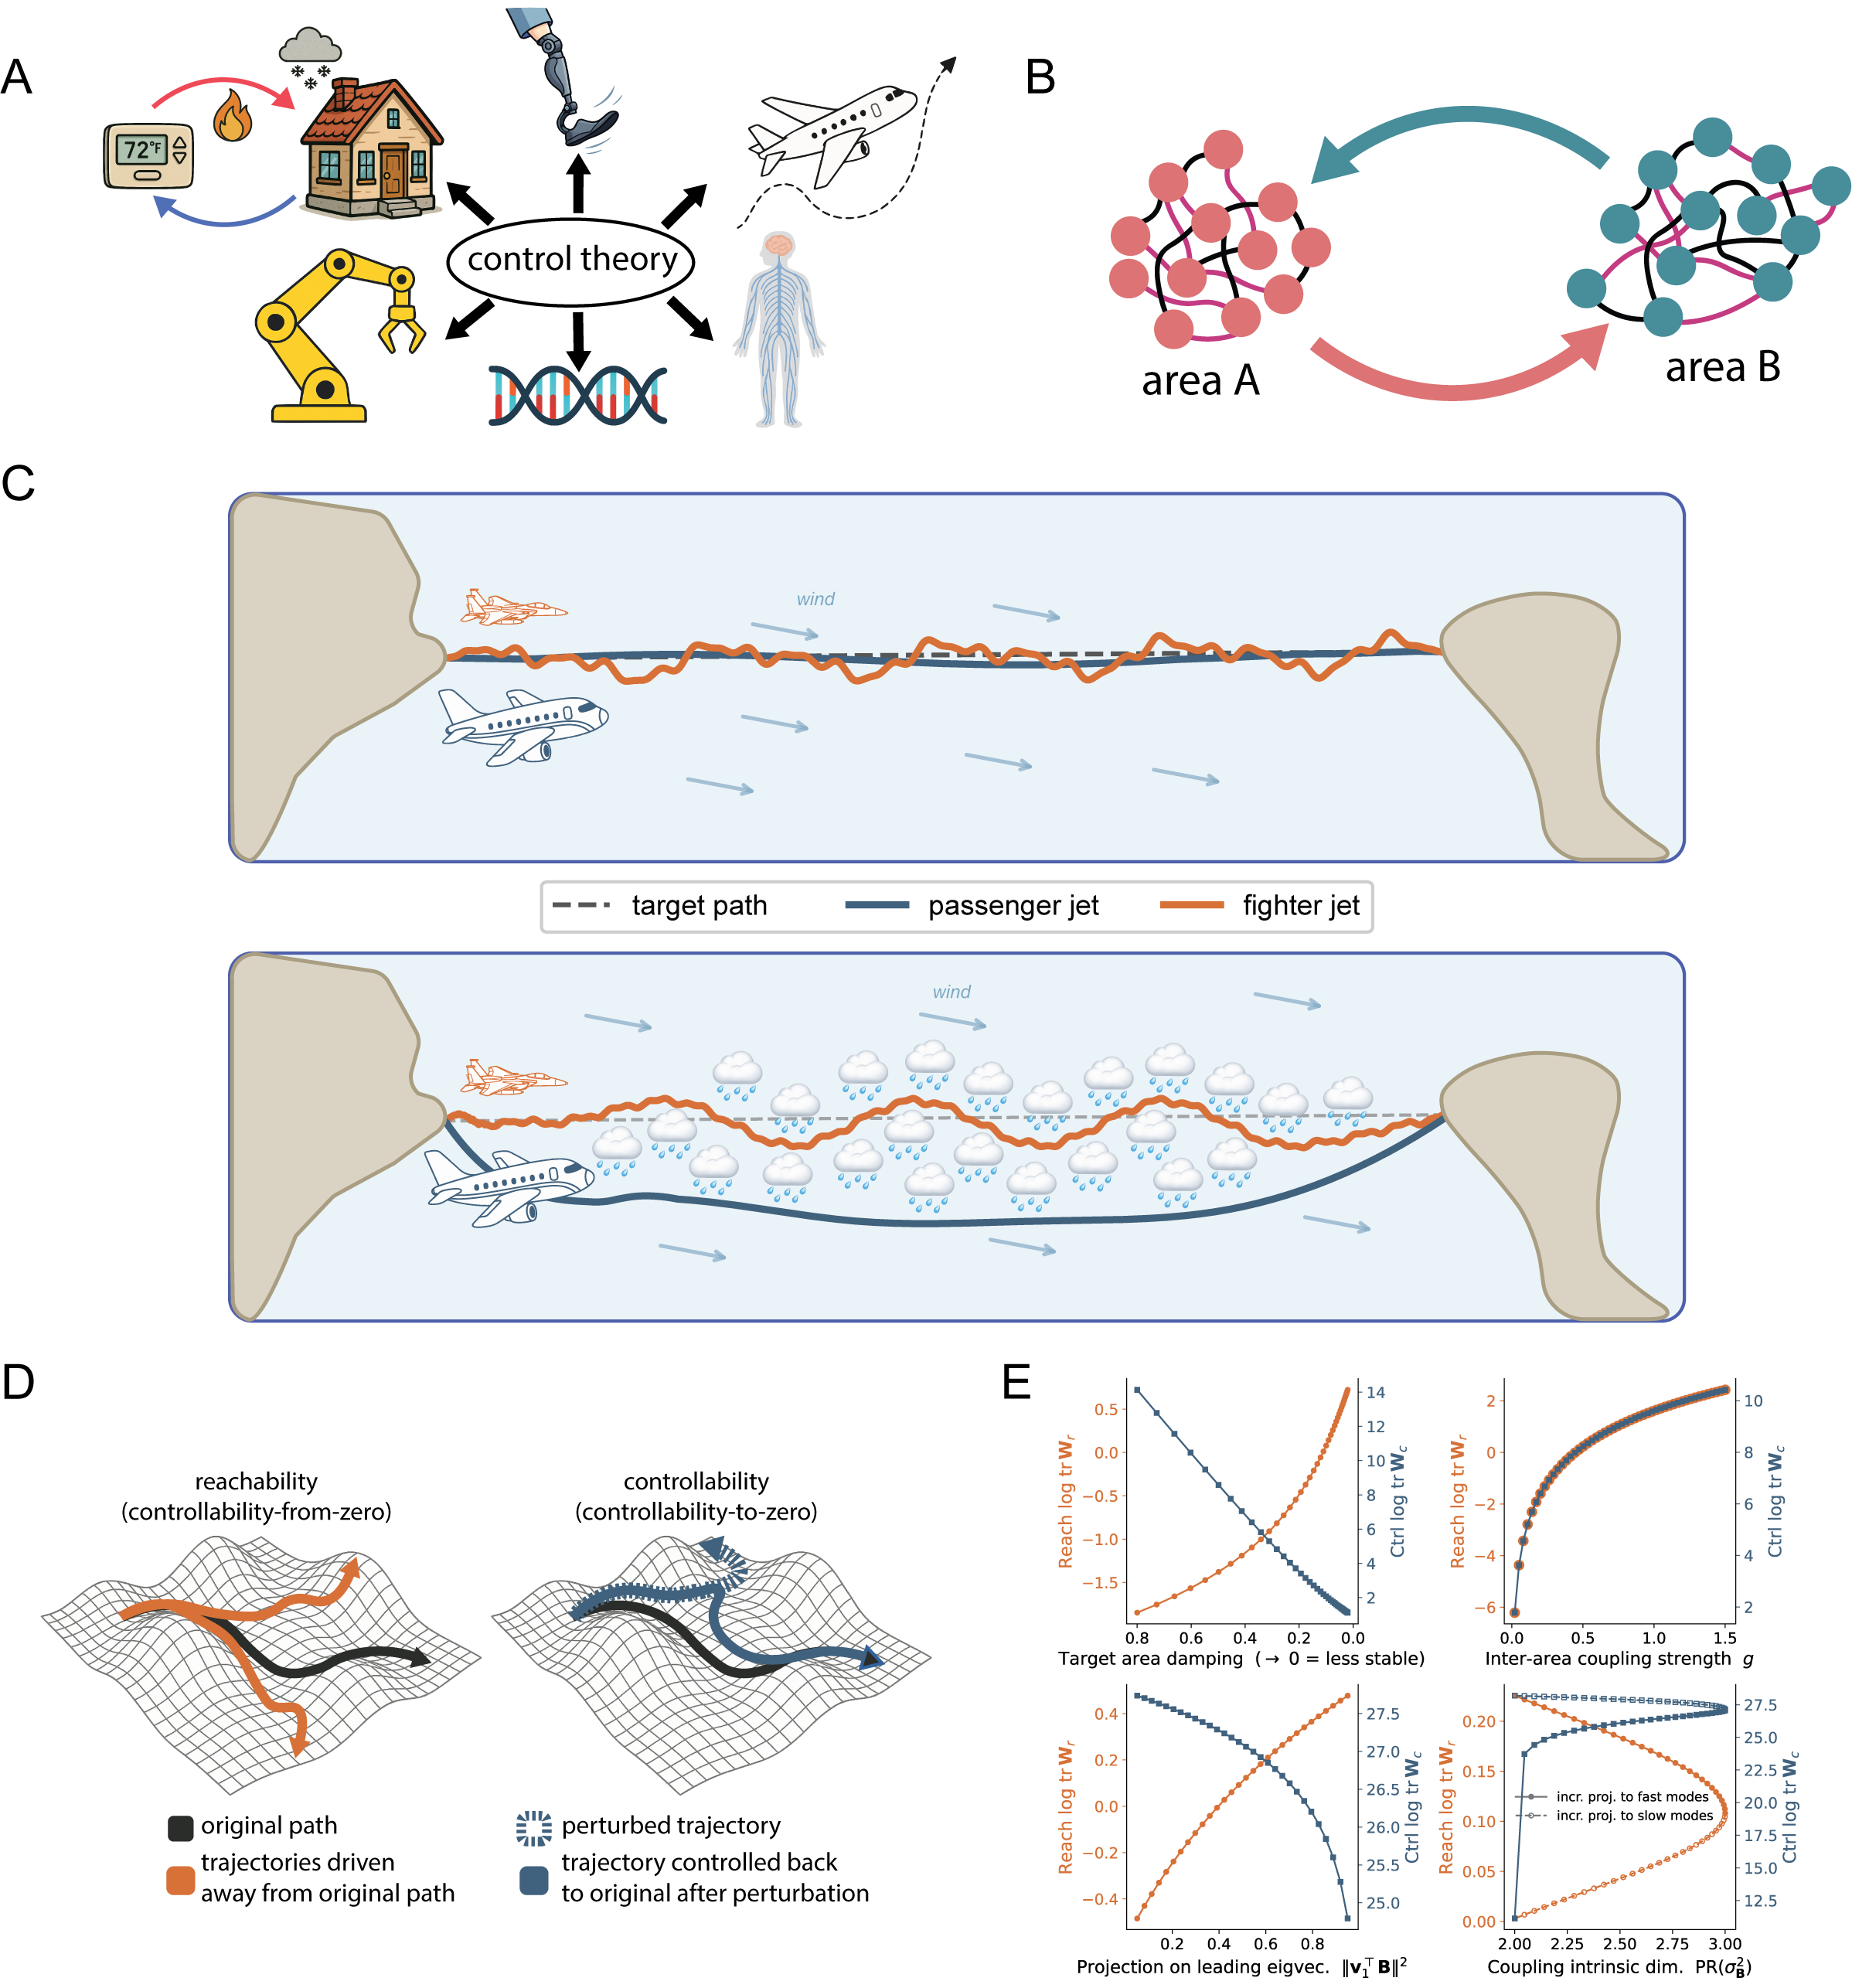
\includegraphics[width=0.95\linewidth]{figures/interareal-control/fig_introduction.png}
\caption[A control theoretic framing of interareal control.]{\textbf{A control theoretic framing of interareal control.} (A) Control problems share a common formal structure across engineering, biology, and brain networks. (B) Bidirectional control interactions between two areas. (C) Conceptual illustration of reachability and controllability interacting with dynamic stability. (D) Abstract illustration of reachability and controllability. (E) The dependence of reachability and controllability on dynamic stability, coupling magnitude, coupling alignment, and coupling dimensionality in a synthetic two-area linearization.}
\label{fig:interareal-control-introduction}
\end{figure}

\section{Jacobian-based directional control estimation}
\label{sec:interareal-control-methods}

We consider nonlinear dynamical systems in $\mathbb{R}^d$. The full system is defined by the dynamics $\dot{\vb{u}}(t) = \vb{f}(\vb{u}(t))$. We assume that within this full system, there are $K$ coupled subsystems, each of which is defined by the dynamics $\dot{\vb{u}}^k(t) = \vb{f}^k(\vb{u}(t))$, $k = 1, \ldots, K$. The subsystem dimensionalities are $d_k$, and $d = \sum_{k=1}^{K} d_k$. The system is then observed through a smooth map $\vb{x}(t)=\vb{h}(\vb{u}(t))\in\mathbb{R}^{d_{\mathrm{obs}}}$ with $\vb{h}: \mathbb{R}^d \to \mathbb{R}^{d_{\mathrm{obs}}}$ that projects the full state vector $\vb{u}$ onto a lower-dimensional subspace. We will assume that our observation of each subsystem depends only on the state of the subsystem itself, and not on the state of the other subsystems. That is, we can decompose the observation map as $\vb{x}(t) = \vb{h}(\vb{u}(t)) = [\vb{h}^1(\vb{u}^1(t)), \vb{h}^2(\vb{u}^2(t)), \ldots, \vb{h}^K(\vb{u}^K(t))]$.

\subsection{Jacobian-based directional control estimation in fully observed dynamical systems}

We begin with the simplest case discussed in the original JacobianODE paper~\cite{Eisen2025-wt}, when $\vb{h}$ is the identity map, so $\vb{x}(t) = \vb{u}(t)$. The Jacobian of the dynamics is a matrix-valued function $\mathbf{J}_\mathbf{f}: \mathbb{R}^d \to \mathbb{R}^{d \times d}$ (henceforth, $\mathbf{J}$) given by

\begin{equation}
\mathbf{J}(\mathbf{x}(t)) = \frac{\partial }{\partial \mathbf{x}}\mathbf{f}(\mathbf{x}(t)) =
\begin{bmatrix}
\frac{\partial f_1 }{\partial x_1}& \frac{\partial f_1}{\partial x_2} & \dots & \frac{\partial f_1}{\partial x_d} \\
\frac{\partial f_2 }{\partial x_1}& \frac{\partial f_2}{\partial x_2} & \dots & \frac{\partial f_2}{\partial x_d} \\
\vdots & \vdots & \ddots & \vdots \\
\frac{\partial f_d }{\partial x_1}& \frac{\partial f_d}{\partial x_2} & \dots & \frac{\partial f_d}{\partial x_d} \\
\end{bmatrix}.
\end{equation}

At each time $t$, the Jacobian captures how perturbations to the system will propagate. This recasts nonlinear dynamics as linear time-varying dynamics in the tangent space locally along trajectories (formally, $\delta\dot{\mathbf{x}}(t) = \mathbf{J}_\mathbf{f}(\mathbf{x}(t)) \delta \mathbf{x}(t)$) (Figure~\ref{fig:interareal-control-methods}A, left).

\begin{figure}[ht!]
\centering
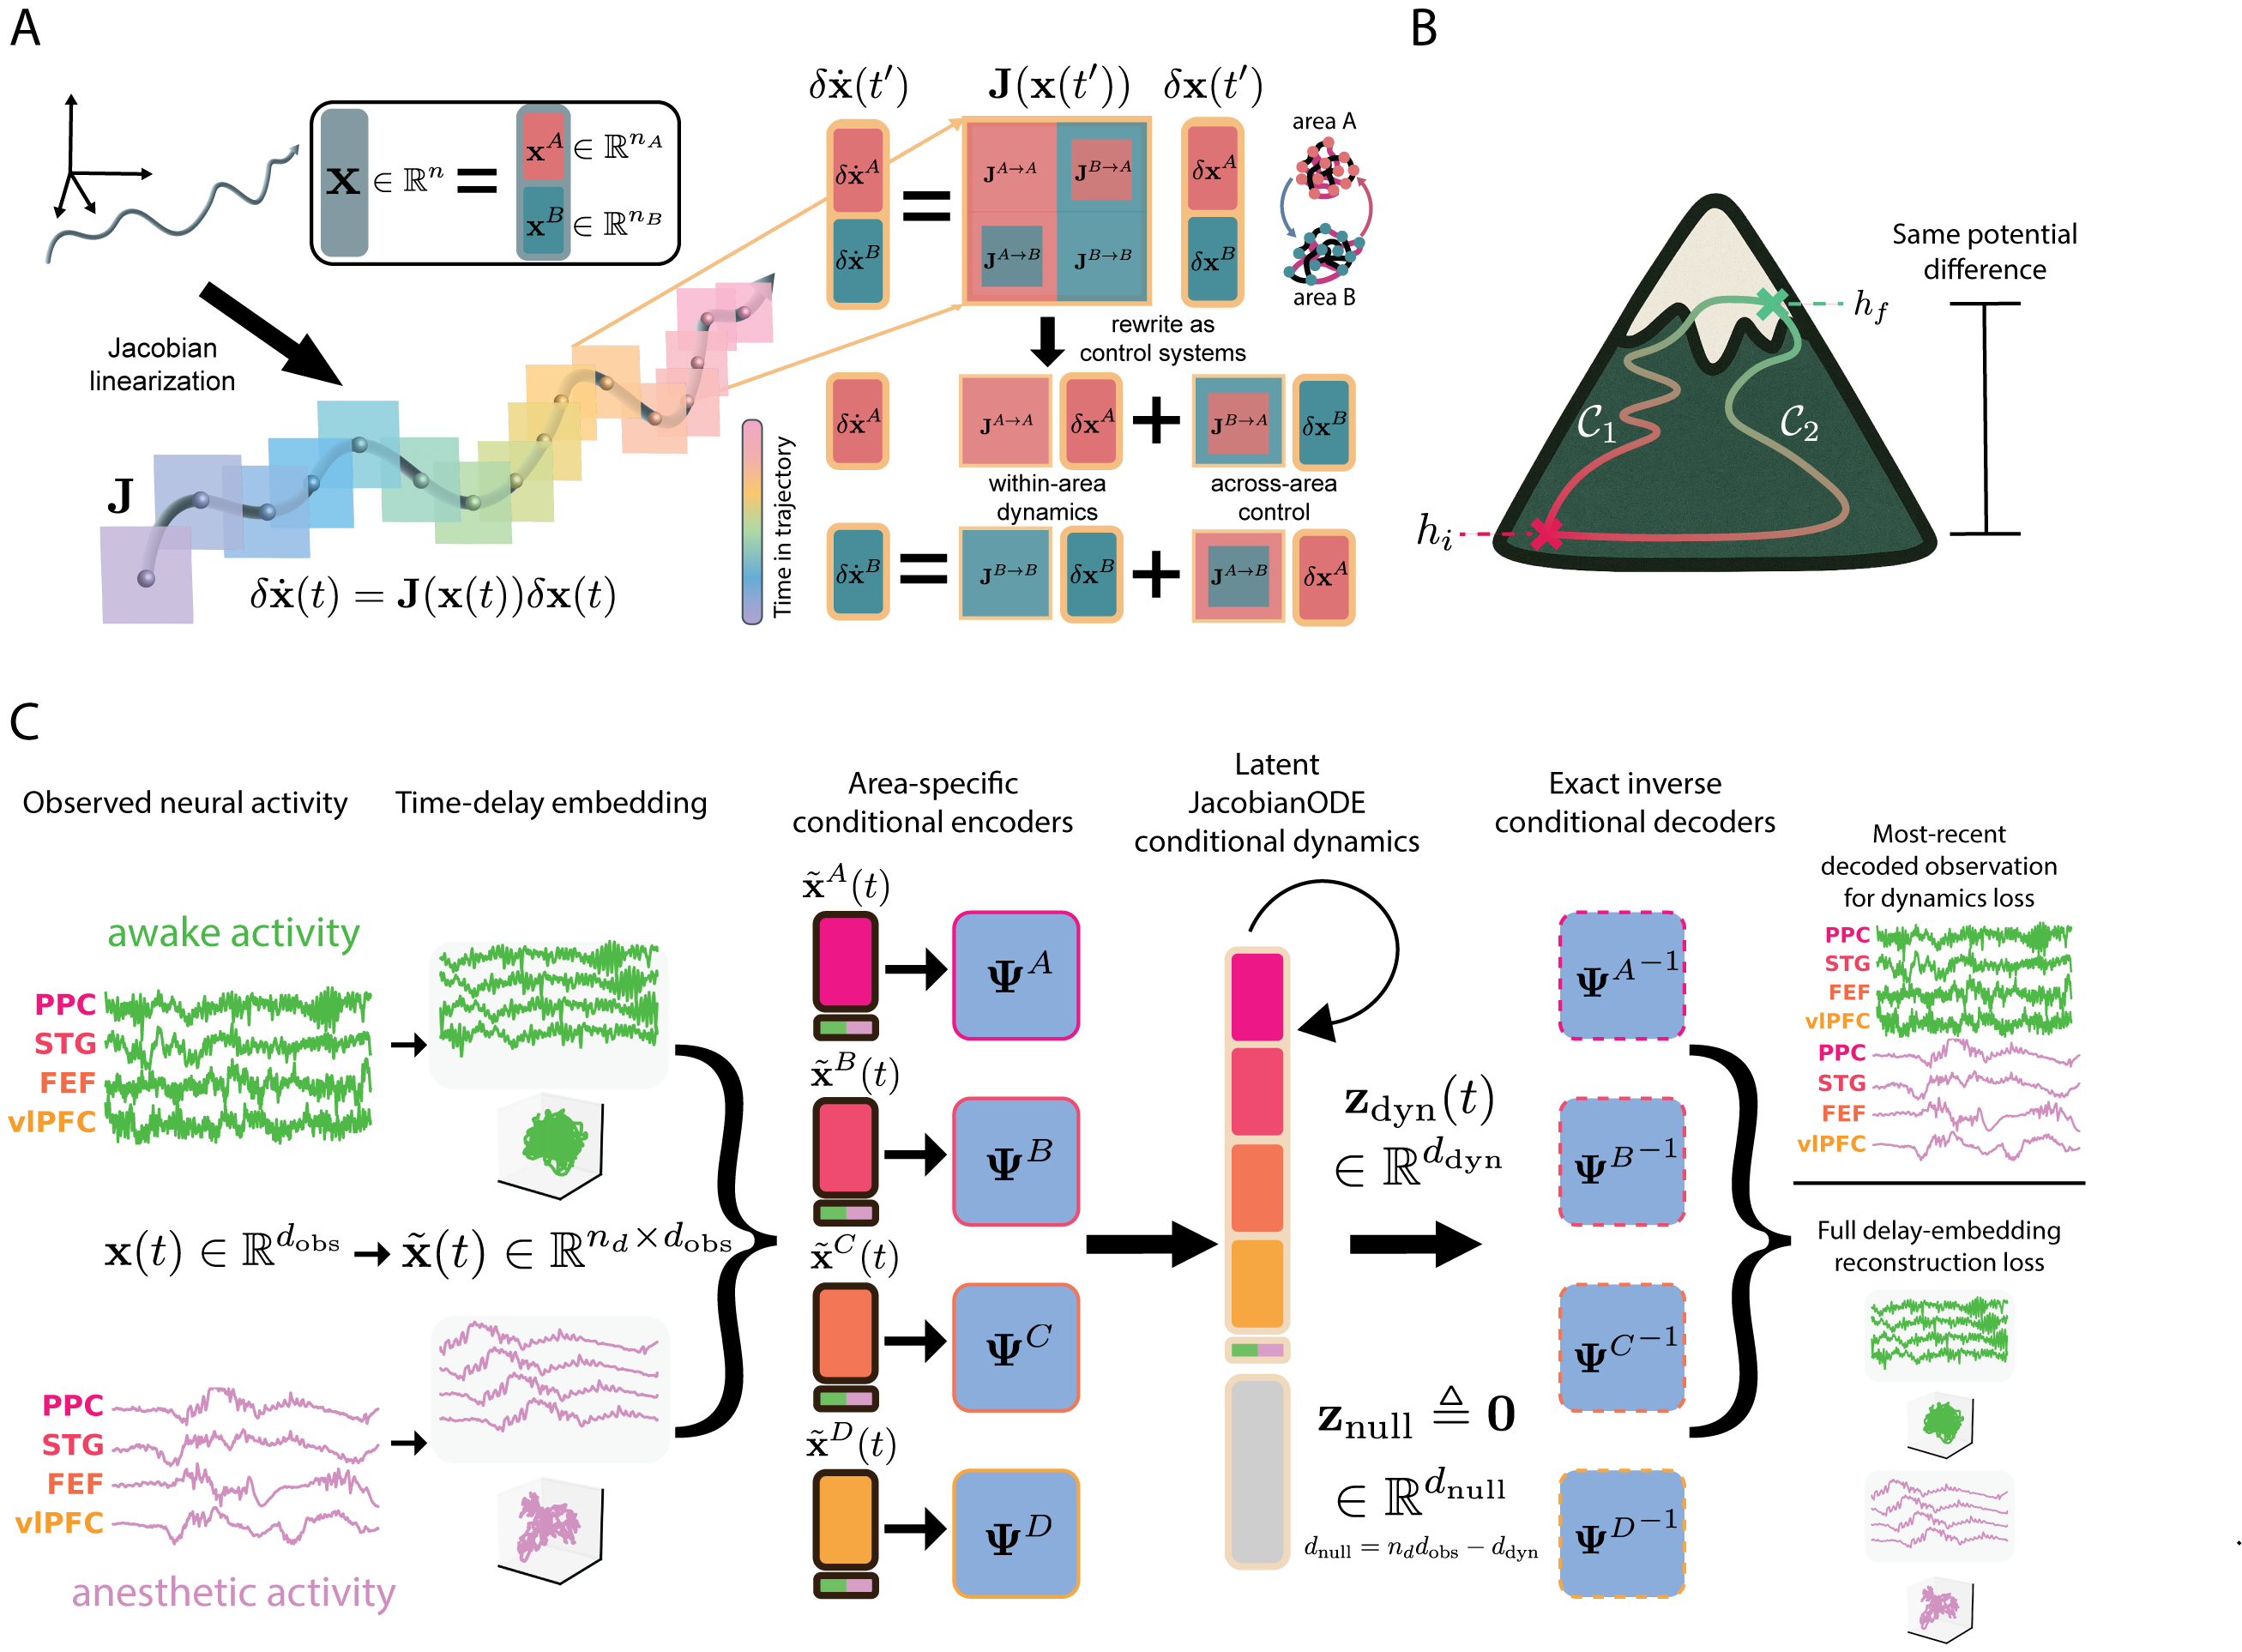
\includegraphics[width=0.95\linewidth]{figures/interareal-control/fig_methods.png}
\caption[Latent JacobianODE pipeline for partially observed multi-area neural recordings]{\textbf{Latent JacobianODE pipeline for partially observed multi-area neural recordings.} (A) Jacobians linearize dynamics along a reference trajectory, enabling the construction of pairwise interacting control systems. (B) Jacobians obey path independence, analogous to achieving the same potential energy difference taking two different paths up a mountain with the same endpoints. (C) The latent JacobianODE deep learning framework, demonstrated using the four-area neural recordings analyzed in this work.}
\label{fig:interareal-control-methods}
\end{figure}

To characterize control, consider the following formulation. As discussed in the original JacobianODE paper, the tangent space dynamics around the reference trajectory for subsystem $\alpha \in \{1,...,K\}$ are given by \[
\delta \dot{\mathbf{x}}^{(\alpha)}(t) = \sum_{k=1}^{K} \mathbf{J}^{k\to\alpha}(\mathbf{x}(t))\delta\mathbf{x}^{(k)}(t)
\] where $\mathbf{J}^{k\to\alpha}(\mathbf{x}(t)) \in \mathbb{R}^{d_{\alpha}\times d_k}$ is the submatrix of $\mathbf{J}(\mathbf{x}(t))$ in which the columns correspond to subsystem $k$ and the rows correspond to subsystem $\alpha$. Now, for a given subsystem $\beta \in \{1, ..., K\}$ with $\beta \neq \alpha$, we wish to analyze the ease with which $\beta$ can control $\alpha$ locally around the reference trajectory, without intervention from other subsystems. Discounting the interventions from other subsystems equates to setting $\delta\mathbf{x}^{(k)}(t) = 0$ for $k \neq \alpha,\beta$, leaving the expression
\begin{equation}
\delta \dot{\mathbf{x}}^{(\alpha)}(t) =\mathbf{J}^{\alpha\to\alpha}(\mathbf{x}(t))\delta\mathbf{x}^{(\alpha)}(t) + \mathbf{J}^{\beta\to\alpha}(\mathbf{x}(t))\delta\mathbf{x}^{(\beta)}(t)
\end{equation}
which quantifies the influence $\beta$ can exert over $\alpha$ in the absence of perturbations from any other subsystem (Figure~\ref{fig:interareal-control-methods}A, right). Using this representation, the reachability Gramian can be computed as described above. Performing this procedure for all pairs of subsystems $\alpha,\beta \in \{1,...,K\}$ thus characterizes all pairwise control relationships between subsystems along the reference trajectory.

To characterize control, we can use the reachability and controllability Gramians, defined in continuous time as

\begin{equation}
\mathbf{W}_r(t_0, t_1) \triangleq \int_{t_0}^{t_1}\mathbf{\Phi}(t_1, \tau)\mathbf{B} (\tau)\mathbf{B}^T(\tau){\mathbf{\Phi}}^T(t_1, \tau) d\tau
\end{equation}

and

\begin{equation}
\mathbf{W}_c(t_0, t_1) \triangleq \int_{t_0}^{t_1}\mathbf{\Phi}(t_0, \tau)\mathbf{B} (\tau)\mathbf{B}^T(\tau){\mathbf{\Phi}}^T(t_0, \tau) d\tau
\end{equation}

respectively. In these equations, $\mathbf{\Phi}$ denotes the state-transition matrix of the intrinsic dynamics of subsystem $\alpha$ without any input (i.e., $\delta\mathbf{x}^{(\alpha)}(t) = \mathbf{\Phi}(t, t_0)\delta\mathbf{x}^{(\alpha)}(t_0)$) and $B$ denotes the coupling Jacobian $\mathbf{J}^{\beta\to\alpha}(\mathbf{x}(t))$.\cite{Antsaklis2006-wl}

\subsection{Deep Jacobian estimation: learning Jacobians from data}

Given only observed trajectories $\vb{x}^{(j)}(t_0^{(j)} + k\Delta t)$, $k=0,1,\dots$, and no access to the underlying dynamics $\vb{f}$, we estimate $\mathbf{J}$ directly by parameterizing it as a neural network $\hat{\mathbf{J}}^{\theta}$ with learnable parameters $\theta$, trained on observed data following the JacobianODE method.\cite{Eisen2025-wt} The core observation is that each row of $\mathbf{J}$ is a conservative vector field (the gradient of a scalar potential), so its path integral between any two points is path-independent~\cite{Lorraine2024-qe,Beik-Mohammadi2024-mg}: as in the work done climbing a mountain, the result depends only on the start and end points, not the route taken (Figure~\ref{fig:interareal-control-methods}B). Formally,
\begin{equation}
\vb{f}(\vb{x}(t_f)) - \vb{f}(\vb{x}(t_i)) \ =\ \int_{\mathcal{C}}\hat{\mathbf{J}}^{\theta}\, d\vb{s},
\label{eq:interareal-control-pathint}
\end{equation}
where $\mathcal{C}$ is any piecewise-smooth curve joining $\vb{x}(t_i)$ to $\vb{x}(t_f)$. Together with a Jacobian-based parameterization of the reference value $\vb{f}(\vb{x}(t_i))$ so that all gradients backpropagate through $\theta$ (see Appendix~\ref{supp:interareal-control-proof-Fjac}), Equation~\ref{eq:interareal-control-pathint} yields an estimate of the time derivative everywhere along the trajectory, which a standard ODE integrator advances to predict $\hat{\vb{x}}(t_f + \Delta t)$.

\insettitle{Trajectory loss.} Given an observed trajectory $\vb{x}(t_0 + k\Delta t)$, $k=0,\dots,T-1$, the trajectory reconstruction loss $\mathcal{L}_{\mathrm{traj}}(\theta;\vb{x})$ penalizes deviation between predicted and true states under an appropriate distance (typically mean squared error, i.e. MSE). Recursive predictions in chaotic or noisy systems are stabilized by generalized teacher forcing, which partially anchors the rollout to ground-truth states.\cite{Hess2023-kp}

\insettitle{Loop-closure loss.} Trajectory loss only constrains $\hat{\mathbf{J}}^{\theta}$ along the direction of the flow, leaving the orthogonal tangent-space directions underdetermined. Exploiting conservativity once more, the path integral of $\mathbf{J}$ around any piecewise-smooth closed loop $\mathcal{C}_{\mathrm{loop}}$ must vanish (Figure~\ref{fig:interareal-control-methods}C). The self-supervised loop-closure regularizer~\cite{Iyer2024-kk},
\begin{equation}
\mathcal{L}_{\mathrm{loop}}(\theta;\vb{x}) \ =\ \Big\|\oint_{\mathcal{C}_{\mathrm{loop}}}\hat{\mathbf{J}}^{\theta}\, d\vb{s}\Big\|_2^{2},
\label{eq:interareal-control-loopclosure}
\end{equation}
penalizes departure from zero over loops formed from concatenations of line segments between randomly-sampled data points, sampling diverse tangent-space directions on the data manifold while remaining cheap to compute.

\insettitle{Training objective.} The total loss combines the two terms,
\begin{equation}
\mathcal{L}(\theta;\vb{x}) \ =\ \mathcal{L}_{\mathrm{traj}}(\theta;\vb{x}) + \lambda_{\mathrm{loop}}\,\mathcal{L}_{\mathrm{loop}}(\theta;\vb{x}),
\label{eq:interareal-control-jacobianode-loss}
\end{equation}
with $\lambda_{\mathrm{loop}}$ a tunable hyperparameter controlling the weight of the loop-closure regularizer.

\subsection{A latent JacobianODE pipeline for partially observed dynamical systems}

\insettitle{Delay embedding.} To recover the full system dynamics from partial observations, we can leverage Takens' delay embedding theorem. The theorem guarantees that by looking backwards in time at the history of the observed data, we can reconstruct a manifold that is diffeomorphic to the full system state space. Specifically, we form delay-embedded vectors $\tilde{\vb{x}}(t) = [\vb{x}(t), \vb{x}(t-\tau\Delta t), \ldots, \vb{x}(t-(n_d-1)\tau\Delta t)] \in \mathbb{R}^{d'}$, with $d' = n_d d_{\mathrm{obs}}$. Takens' theorem guarantees that for generic $\vb{h}$ and $n_d \geq 2d^{\star} + 1$, the map $\tilde{\vb{x}} \mapsto \vb{u}$ is a diffeomorphism from the embedded manifold onto the full system state space. We will again assume subsystem-specificity of the observation map, so that $\tilde{\vb{x}}(t)$ can be written as $\tilde{\vb{x}}(t) = [\tilde{\vb{x}}^1(t); \tilde{\vb{x}}^2(t); \ldots; \tilde{\vb{x}}^K(t)] \in \mathbb{R}^{d'}$, and the diffeomorphism is given by $\vb{u} = \vb{\psi}(\tilde{\vb{x}}) = [\vb{\psi}^1(\tilde{\vb{x}}^1(t)); \vb{\psi}^2(\tilde{\vb{x}}^2(t)); \ldots; \vb{\psi}^K(\tilde{\vb{x}}^K(t))]$.

\insettitle{Diffeomorphic encoder.} The latent version of the JacobianODE model builds on the insight from Takens' theorem, and following previous work,\cite{Versteeg2023-ld} leverages diffeomorphic encoders to learn a latent representation that is diffeomorphic to the delay embedding. Specifically, we delay embed the observed data, and construct an encoder that consists of coupling layers interleaved with orthogonal mixing layers. This results in an encoder that is both diffeomorphic and exactly invertible (Figure~\ref{fig:interareal-control-methods}C, left). In practice, we use additive coupling layers for the coupling component, and Cayley-parameterized orthogonal mixers for the mixing component.\cite{Dinh2014-lx,Lezcano-Casado2019-su,Trockman2021-iw} Formally, an invertible additive coupling layer takes as input a vector $\vb{y} \in \mathbb{R}^{d'}$, partitions it into two halves $\vb{a} \in \mathbb{R}^{d'/2}$ and $\vb{b} \in \mathbb{R}^{d'/2}$, and applies

\begin{equation}
\vb{a}' = \vb{a}, \qquad \vb{b}' = \vb{b} + \vb{m}_\vartheta(\vb{a}),
\end{equation}
where $\vb{m}_\vartheta:\mathbb{R}^{d'/2} \to \mathbb{R}^{d'/2}$ is a (possibly non-invertible) neural network. The Jacobian of this map is

\begin{equation}
\frac{\partial(\vb{a}',\vb{b}')}{\partial(\vb{a},\vb{b})} = \begin{bmatrix} \mathbf{I} & \mathbf{0} \\ \nabla_{\!\vb{a}}\,\vb{m}_\vartheta & \mathbf{I} \end{bmatrix},
\end{equation}
which has $\det = 1$ identically, regardless of $\vb{m}_\vartheta$. The inverse is $\vb{a} = \vb{a}'$, $\vb{b} = \vb{b}' - \vb{m}_\vartheta(\vb{a}')$, computable in one forward pass.

To mix the dimensions in between coupling layers, we use a Cayley-parameterized orthogonal mixer. Formally, a Cayley-parameterized orthogonal mixer takes as input a vector $\vb{y} \in \mathbb{R}^{d'}$ and applies an orthogonal map given by $\vb{y}' = \vb{Q}\vb{y}$, where $\vb{Q} = (\mathbf{I}-\mathbf{A})(\mathbf{I}+\mathbf{A})^{-1}$ and $\mathbf{A}$ is a learnable skew-symmetric matrix. The determinant of $\vb{Q}$ is 1.

Thus the encoder as a whole is volume preserving (its determinant is 1), meaning it cannot arbitrarily reduce the geometric volume of the observed data to minimize noise. To handle multiple subsystems, we instantiate a separate encoder for each subsystem, so that the total encoder can be written as $\vb{z} = \vb{\Psi}(\tilde{\vb{x}}(t)) = [\vb{\Psi}^1(\tilde{\vb{x}}^1(t)); \vb{\Psi}^2(\tilde{\vb{x}}^2(t)); \ldots; \vb{\Psi}^K(\tilde{\vb{x}}^K(t))]$.

A diffeomorphic function by construction must map to a space of the same dimensionality. However the intrinsic dimensionality of a system is in practice typically much smaller than the dimension of the delay embedding. We partition the latent space into two components: a dynamic latent $\mathbf{z}_{\mathrm{dyn}} \in \mathbb{R}^{d_{\mathrm{dyn}}}$ and an effectively-null latent $\mathbf{z}_{\mathrm{null}} \in \mathbb{R}^{d_{\mathrm{null}}} = \mathbb{R}^{n_d d_{\mathrm{obs}} - d_{\mathrm{dyn}}}$, with $\vb{z} = [\vb{z}_{\mathrm{dyn}}; \vb{z}_{\mathrm{null}}] \in \mathbb{R}^{n_d d_{\mathrm{obs}}}$ (Figure~\ref{fig:interareal-control-methods}C, center). The null subspace is zero-padded for all decoder calls (i.e., inverse encoder calls). Thus while the null subspace is allowed to freely vary, all information for both dynamics and reconstruction must live in the dynamic latent. The JacobianODE model then operates on $\mathbf{z}_{\mathrm{dyn}}$ only. Note that since the encoder is volume-preserving, as mentioned, all information in the input must be preserved \textit{somewhere} in the latent space. Thus the null subspace provides the opportunity to dump any noise or information not relevant to the dynamics or reconstruction. In practice, to pick the dimensionality of the dynamic subspace $d_{\mathrm{dyn}}$, we perform a linear PCA on the delay-embedded training data and select the number of components that explain 99\% of the variance. This is because linear dimensionality provides an upper bound on the intrinsic dimensionality of the system.

\insettitle{Reconstruction loss.} The reconstruction loss $\mathcal{L}_{\mathrm{rec}}(\theta_{\Psi};\vb{x})$ penalizes the deviation between true and decoded latent states, where $\theta_{\Psi}$ are the parameters of the encoder (Figure~\ref{fig:interareal-control-methods}C, right). We define a projection operator $P_{\text{dyn}}$ that projects the latent into the dynamic subspace. Then, the reconstruction loss is given by

\begin{equation}
\mathcal{L}_{\mathrm{rec}}(\theta_{\Psi};\vb{x}) = \mathbb{E}_t\big[\|\vb{\Psi}^{-1}\left([P_{\text{dyn}}\vb{\Psi}(\tilde{\vb{x}}(t)); \mathbf{0}]\right) - \vb{\tilde{x}}(t)\|^2\big].
\label{eq:interareal-control-reconstruction-loss}
\end{equation}

\insettitle{Latent prediction loss.} The latent prediction loss $\mathcal{L}_{\mathrm{pred}, \mathbf{z}}(\theta;\vb{x})$ penalizes the deviation between true and predicted latent dynamics, where $\theta = [\theta_\Psi; \theta_J]$ are the parameters of the encoder and JacobianODE model. Formally,

\begin{equation}
\mathcal{L}_{\mathrm{pred}, \mathbf{z}}(\theta;\vb{x}) = \mathbb{E}_t\left[\sum_{s=1}^T\Big\|\hat{\vb{z}}(t+s\Delta t) - \vb{z}(t+s\Delta t)\Big\|^2\right],
\label{eq:interareal-control-latent-dynamics-loss}
\end{equation}

where $\hat{\vb{z}}(t+s\Delta t)$ is the predicted latent state at time $t+s\Delta t$ and $T$ is the number of prediction steps.

\insettitle{Decoded prediction loss.} The decoded prediction loss $\mathcal{L}_{\mathrm{pred}, \mathbf{x}}(\theta;\vb{x})$ penalizes the deviation between true and predicted observed states, where $\theta = [\theta_\Psi; \theta_J]$ are the parameters of the encoder and JacobianODE model. To minimize the amount of redundant information, we compute the decoded prediction loss only on the most recent slice of each predicted delay-embedded window (Figure~\ref{fig:interareal-control-methods}C, right). Formally,

\begin{equation}
\mathcal{L}_{\mathrm{pred}, \mathbf{x}}(\theta;\vb{x}) = \mathbb{E}_t\left[\sum_{s=1}^T\Big\|P_{\text{recent}}\vb{\Psi}^{-1}\left([P_{\text{dyn}}\hat{\vb{z}}(t+s\Delta t); \mathbf{0}]\right) - \vb{x}(t+s\Delta t)\Big\|^2\right],
\label{eq:interareal-control-decoded-prediction-loss}
\end{equation}

where $P_{\text{recent}}$ is a projection operator that projects the decoded latent into the most recent slice of the delay-embedded window, and $\vb{x}(t+s\Delta t)$ is the true observed state at time $t+s\Delta t$.

\insettitle{Loop-closure loss.} The loop-closure loss $\mathcal{L}_{\mathrm{loop}}(\theta;\vb{x})$ is computed in latent space, and is given by

\begin{equation}
\mathcal{L}_{\mathrm{loop}}(\theta;\vb{x}) = \mathbb{E}_t\left[\Big\|\oint_{\mathcal{C}_{\mathrm{loop}}}\hat{\mathbf{J}}^{\theta}\, d\vb{s}\Big\|_2^2\right],
\label{eq:interareal-control-loop-closure-loss}
\end{equation}

where $\mathcal{C}_{\mathrm{loop}}$ is a closed loop in latent space.

\insettitle{Training objective.} The total loss is given by

\begin{equation}
\mathcal{L}(\theta;\vb{x}) = \mathcal{L}_{\mathrm{rec}}(\theta_{\Psi};\vb{x}) + \mathcal{L}_{\mathrm{pred}, \mathbf{z}}(\theta;\vb{x}) + \mathcal{L}_{\mathrm{pred}, \mathbf{x}}(\theta;\vb{x}) + \lambda_{\mathrm{loop}}\,\mathcal{L}_{\mathrm{loop}}(\theta;\vb{x}),
\label{eq:interareal-control-total-loss}
\end{equation}

where $\lambda_{\mathrm{loop}}$ is a tunable hyperparameter controlling the weight of the loop-closure regularizer. The reconstruction loss and both prediction losses are given the same weight since the encoder is volume-preserving, and the relevant states should have approximately the same scale.

\subsection{Conditional training}

In the case where the data span multiple conditions, either discrete (e.g., awake vs.\ anesthesia) or continuous (e.g., different drug doses), we can train the JacobianODE model to be condition-aware. Specifically, we can add a conditional vector $\vb{c} \in \mathbb{R}^{d_c}$ to the input of both the encoder and the JacobianODE model, and train the model to predict the Jacobian of the dynamics conditioned on this variable. In practice, we take $c \in \{-1,+1\}$ to represent the difference between conditions.

\section{Results}
\label{sec:interareal-control-results}

\subsection{Validation on synthetic systems with ground-truth dynamics}
\label{sec:interareal-control-validation}

\begin{figure}[ht!]
\centering
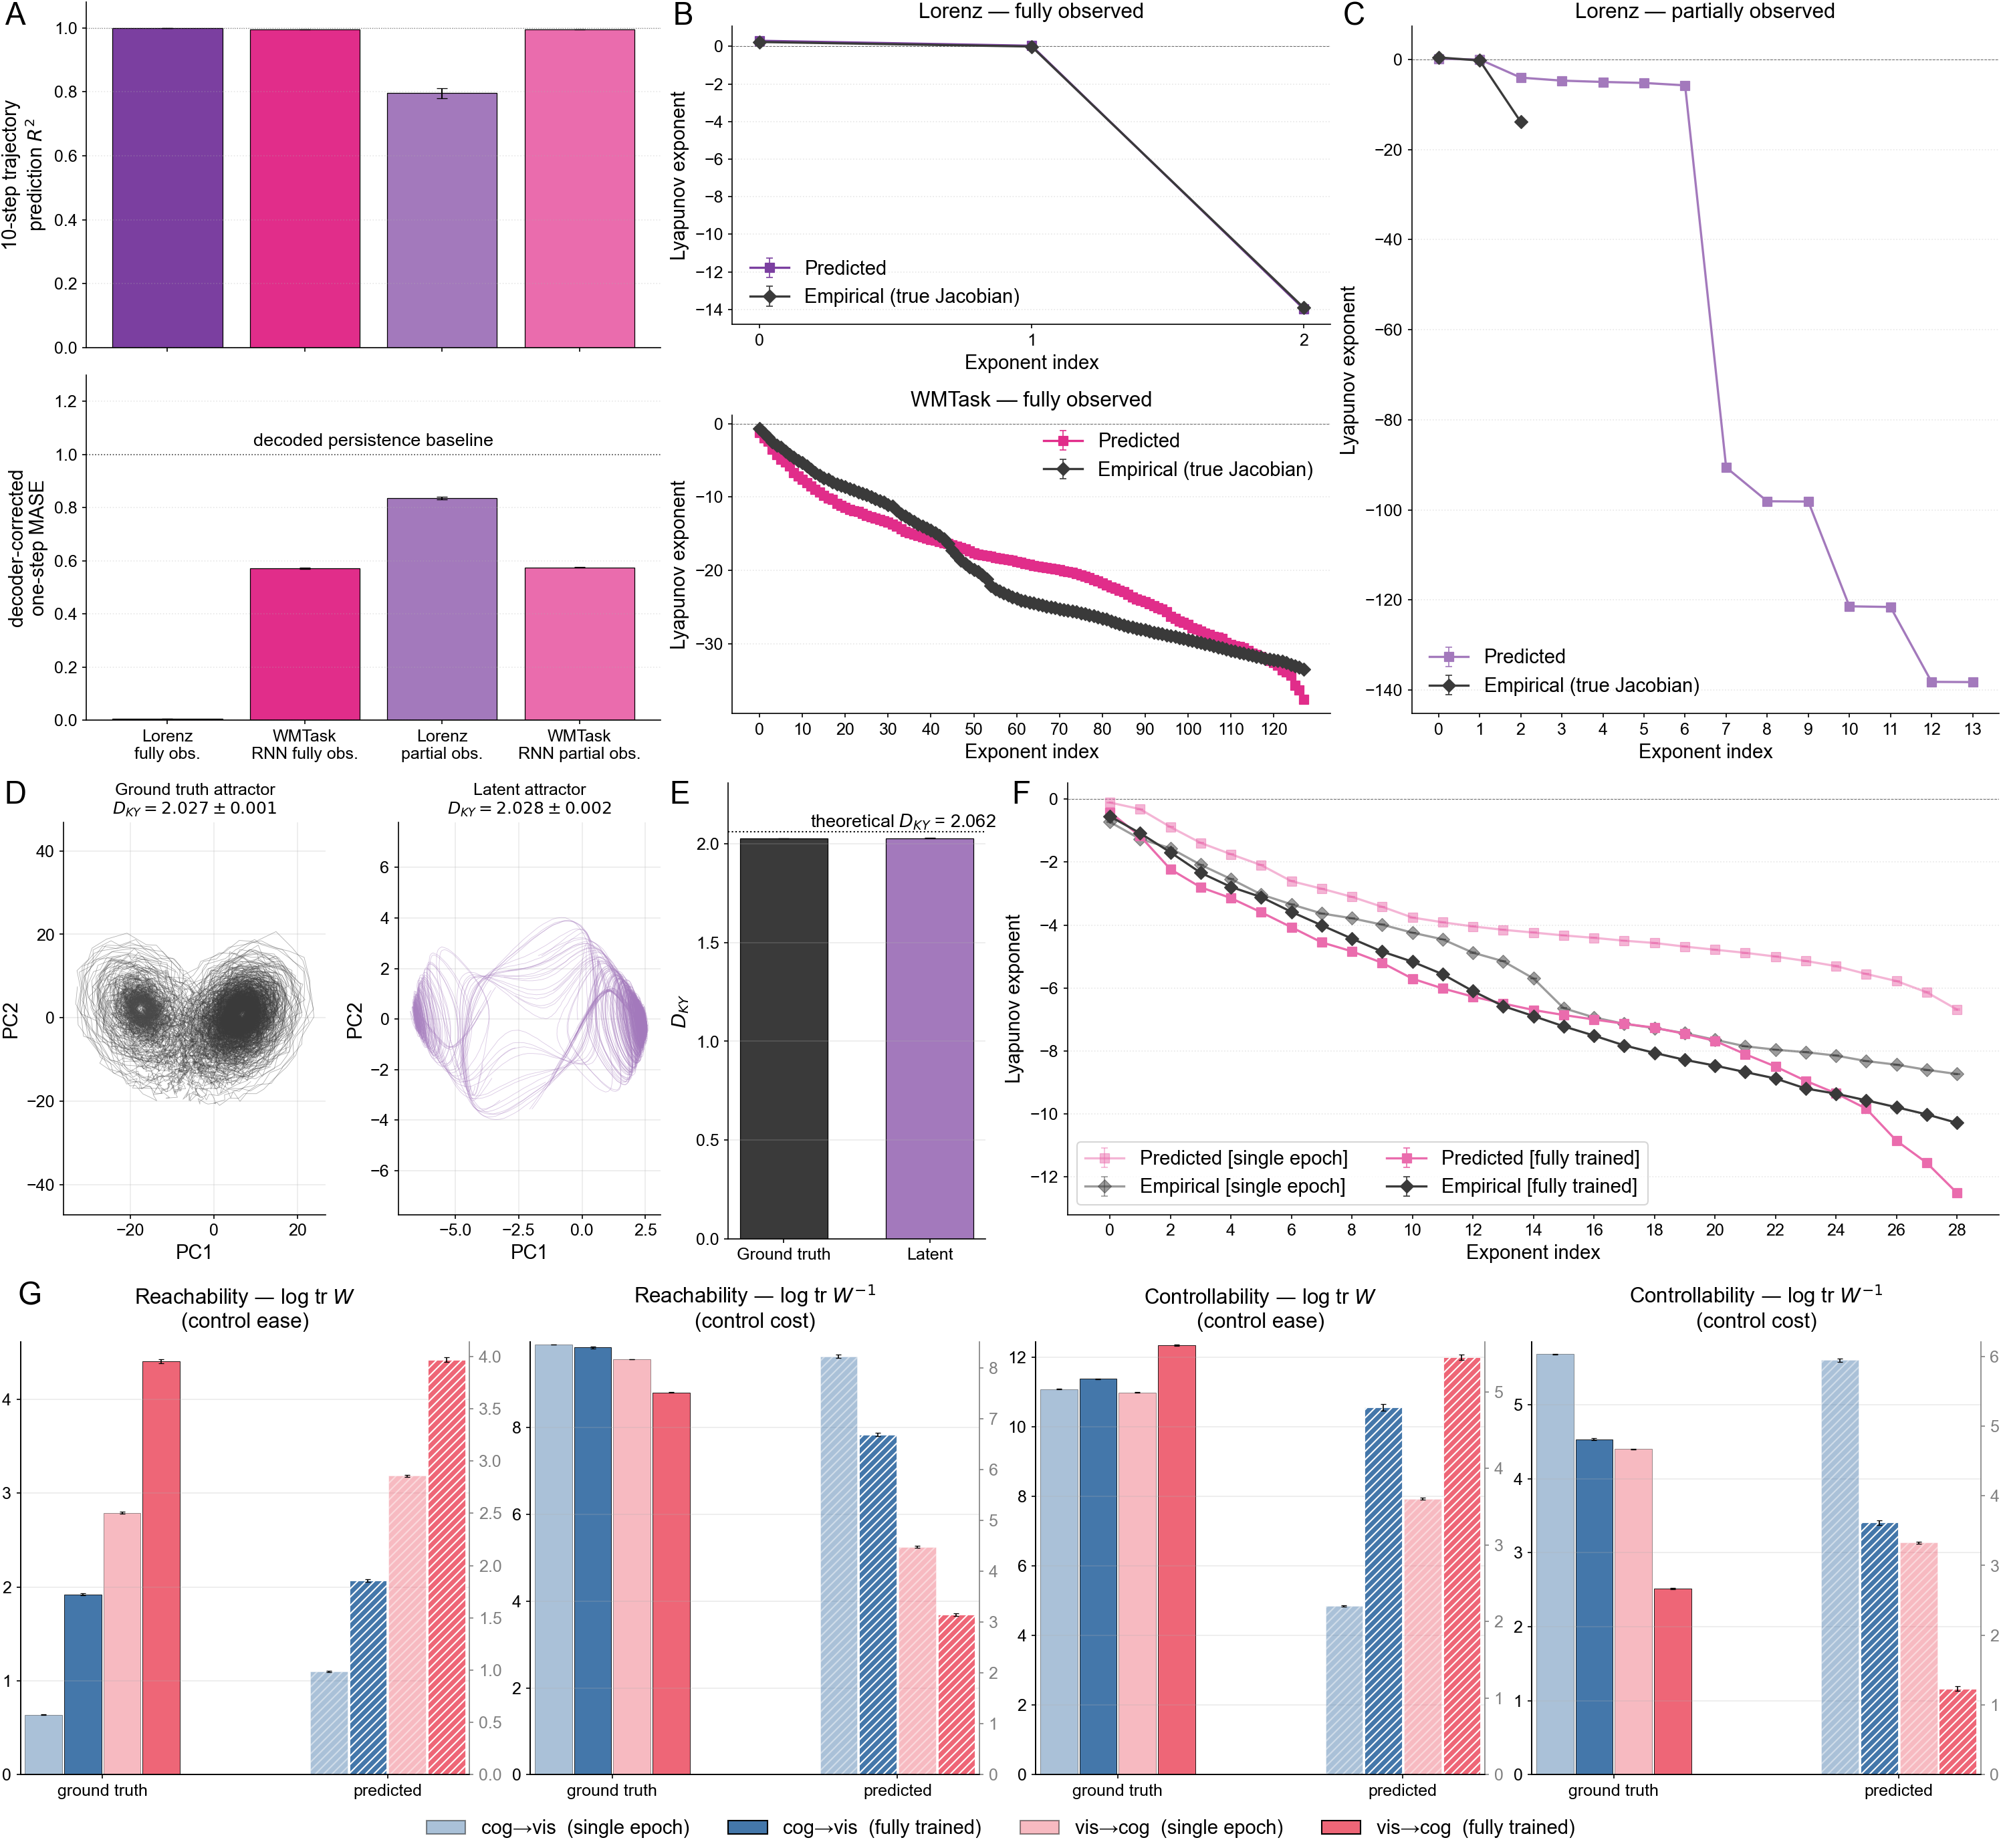
\includegraphics[width=\linewidth]{figures/interareal-control/fig_sample.png}
\caption[Validation on synthetic systems with ground-truth dynamics]{\textbf{Validation on synthetic systems with ground-truth dynamics.} (A)~Ten-step free-running $R^{2}$ (top) and decoder-corrected one-step MASE (bottom) for the four runs. (B)~Predicted vs.\ empirical Lyapunov spectra (sorted descending) for the two fully observed runs. (C)~Same for Lorenz partially observed. (D--E)~Ground-truth and latent-recovered Lorenz attractor in PC1--PC2 with Kaplan--Yorke dimension annotations. (F)~Task-trained RNN single-epoch versus fully trained Lyapunov spectra, predicted (pink) vs.\ empirical (black). (G)~Task-trained RNN partially observed directional reachability and controllability log-trace and inverse log-trace, ground-truth vs.\ predicted, per condition.}
\label{fig:interareal-control-sample}
\end{figure}

We validated the pipeline on two simulated systems. Crucially, in these systems, the true Jacobians are known, so we can compare against ground-truth invariants such as the Lyapunov spectrum, attractor topology, and ground-truth reachability and controllability gramians. The systems we used were the 3-D Lorenz attractor,\cite{Lorenz1963-ho} and a 128-D recurrent neural network (RNN) trained on a working memory selection task inspired by \textcite{Panichello2021-xi}. For the task-trained RNN, on each trial, the network receives two cue inputs and, after a delay and a selection cue, must sustain activation corresponding to the chosen color. The RNN consists of two 64-neuron areas (visual input and cognitive output), with predominantly within-area connectivity to encourage multi-area functional structure. Inputs reach only the visual area, outputs are read from the cognitive area, and thus the two areas are forced to interact to solve the task. We trained Jacobians on activity only from the autonomous delay epoch before the network provides a response.\cite{Eisen2025-wt}

Each system was trained in two variants: fully observed (the JacobianODE machinery receives all $d$ state coordinates) and partially observed (the latent-space pipeline receives a $d_{\mathrm{obs}}\!\ll\!d$ projection and recovers a coordinate system via delay embedding and the coupling encoder). For the Lorenz system, only the $x$ variable was observed, and 16 randomly chosen dimensions from each of the two areas were observed for the task-trained RNN. All systems were trained with 5\% observation noise.

We evaluated trajectory prediction via $R^2$ and decoder-corrected mean absolute standardized error (MASE). The decoder-corrected MASE normalizes the mean absolute error by the absolute error of the decoded persistence baseline ($\mathbb{E}_t\big[\|P_{\text{recent}}\vb{\Psi}^{-1}\left([P_{\text{dyn}}\vb{\Psi}(\tilde{\vb{x}}(t)); \mathbf{0}]\right) - \vb{x}(t + \Delta t)\|^2\big]$), which separates the dynamic prediction quality from the decoder error. Trajectory-prediction quality is reported on held out test data (Figure~\ref{fig:interareal-control-sample}A). The fully observed cases recover trajectories well. Under partial observability, the Lorenz $R^{2}$ predictably drops to $0.796\pm 0.015$ and decoder-corrected MASE to $0.835\pm 0.005$, though the prediction metrics indicate the system dynamics are still well-recovered. The task-trained RNN prediction under partial observation is similar to the fully observed case, indicating that the latent geometry tolerates the 16-channel projection well at the prediction level. For both the fully observed Lorenz and task-trained RNN, the latent JacobianODE formulation recovers the Lyapunov spectrum (Figure~\ref{fig:interareal-control-sample}B), indicating that the latent framework retains the capabilities of the vanilla counterpart.

For the partially observed Lorenz system, the latent JacobianODE formulation recovers the top two exponents, while distributing the third exponent, corresponding to decay onto the attractor, into the remaining 12 latent dimensions (Figure~\ref{fig:interareal-control-sample}C). Note that the partially observed latent spectrum has 14 entries due to the method of picking the latent dimension $d_{\mathrm{dyn}}$ by PCA on the delay-embedded training data at variance threshold $0.99$. The results reflect that under partial observation, the encoded delay-embedded states do not contain the necessary resolution to resolve the third exponent exactly. However, the latent JacobianODE does recover the Kaplan-Yorke dimension of the Lorenz attractor, indicating that the attractor topology is preserved (Figure~\ref{fig:interareal-control-sample}D,E).

For the partially observed task-trained RNN, the latent JacobianODE model was trained conditioned on the condition variable $c \in \{-1, +1\}$, indicating the first epoch or the final epoch of training. The latent JacobianODE model qualitatively recovers the leading exponents of the Lyapunov spectrum in each condition, as well as the relevant difference between them (Figure~\ref{fig:interareal-control-sample}F).

Crucially, the latent JacobianODE model also recovers the relative changes in reachability and controllability between the two conditions (Figure~\ref{fig:interareal-control-sample}G). Reachability increases from the first epoch to the final epoch of training for both visual to cognitive control and cognitive to visual control (Figure~\ref{fig:interareal-control-sample}G, left and center-left). Additionally, visual to cognitive reachability is higher in both conditions, reflecting the need for the visual area to drive the cognitive area to make the correct decision. Controllability also increases from the first epoch to the final epoch of training for both visual to cognitive control and cognitive to visual control (Figure~\ref{fig:interareal-control-sample}G, center-right and right).

\subsection{JacobianODE models capture neural dynamics and show more nonlinear geometry in awake state relative to anesthesia}
\label{sec:interareal-control-nhp-trajectory}

We applied the pipeline to multi-area LFP from two non-human primates (NHPs) recorded during propofol infusion. Each session simultaneously recorded LFP from posterior parietal cortex (PPC), superior temporal gyrus (STG, auditory cortex), frontal eye fields (FEF), and ventrolateral prefrontal cortex (vlPFC) at $1$~kHz and low-pass filtered at 80 Hz. We used resting state trajectories for training the JacobianODE model, defined as starting at least 3 seconds after the onset of any external stimulus (either airpuff, or auditory tone). Data was taken from either the awake state or a maintenance dose anesthetic state, and the JacobianODE model was conditioned on the condition variable $c \in \{-1, +1\}$, indicating the state.

Free-running trajectory quality and decoder-corrected one-step MASE are reported per condition, per NHP (Figure~\ref{fig:interareal-control-neural-lyap}A). Trajectories are well captured over 10-step free-running prediction. Anesthetic state trajectories were generally easier to predict than awake state (Hodges--Lehmann (HL) median paired difference anesthesia $-$ awake $\Delta R^{2}=0.068$ [95\% CI $0.060$, $0.071$], paired two-sided Wilcoxon signed-rank $p=9.5\!\times\!10^{-7}$, $n=21$ sessions, all 21/21 positive), though for both conditions the decoder-corrected one-step MASEs are below the decoder-corrected persistence baseline of 1.0.

The encoder leverages considerable transformations to encode the dynamics into the latent space. The angle of rotation rises through the depth of the encoder, and rotates the latent space into a more complex geometry (Figure~\ref{fig:interareal-control-neural-lyap}B). Furthermore, the Riemannian metric induced on the latent space is farther from identity in the awake state than during anesthesia, indicating a more complex geometry in the awake state (Figure~\ref{fig:interareal-control-neural-lyap}C; HL median paired difference anesthesia $-$ awake $\Delta=-0.059$ [95\% CI $-0.067$, $-0.050$], paired two-sided Wilcoxon signed-rank $p=9.5\!\times\!10^{-7}$, $n=21$ sessions, all 21/21 negative). This suggests that the decreased prediction quality in the awake state relative to anesthesia may be related to the more nonlinear geometry of the data manifold.

\subsection{Broad-spectrum destabilization during propofol anesthesia}
\label{sec:interareal-control-lyapunov}

Previous work has shown that neural dynamics are destabilized under propofol anesthesia.\cite{Eisen2024-vc, Eisen2026-cw} We confirmed this destabilization using the latent JacobianODE models.

We computed Lyapunov exponents for all resting state trajectories within each epoch of each session and then averaged across sessions. We report both the asymptotic Lyapunov spectrum as well as the finite time Lyapunov exponent (FTLE) spectrum, computed over 10 millisecond windows.

For the asymptotic Lyapunov exponents, while the largest Lyapunov exponents are similar across conditions, the broad spectrum of Lyapunov exponents is significantly destabilized under anesthesia, as was previously found (Figure~\ref{fig:interareal-control-neural-lyap}D,E; paired two-sided Wilcoxon signed-rank with HL median paired difference, anesthesia $-$ awake, $n=21$ sessions: asymptotic max $\lambda$ $\Delta=-0.59$ [95\% CI $-2.50$, $1.25$], $p=0.59$, 11/21 positive; asymptotic full-spectrum mean $\langle\lambda\rangle$ $\Delta=+5.61$ [95\% CI $+4.56$, $+6.78$], $p=9.5\!\times\!10^{-7}$, all 21/21 positive). For the finite-time Lyapunov exponents, both the maximum Lyapunov exponent and full spectra show destabilizations during anesthesia (Figure~\ref{fig:interareal-control-neural-lyap}D,E; paired two-sided Wilcoxon signed-rank with HL median paired difference, anesthesia $-$ awake, $n=21$ sessions: 10-ms FTLE max $\lambda$ $\Delta=+3.82$ [95\% CI $+0.52$, $+6.97$], $p=0.038$, 13/21 positive; 10-ms FTLE full-spectrum mean $\langle\lambda\rangle$ $\Delta=+5.61$ [95\% CI $+4.56$, $+6.78$], $p=9.5\!\times\!10^{-7}$, all 21/21 positive), suggesting that neural dynamics overall have local expansion followed by global contraction that becomes more pronounced under anesthesia. The near-identical asymptotic and finite-time full-spectrum means follow from the approximate linearity of the learned Jacobians along the trajectory, under which the finite-time and asymptotic Lyapunov exponents largely coincide (Appendix~\ref{supp:interareal-control-linearity}). We note that the maximum Lyapunov exponents are not always faithfully reproduced in the sample systems and may be more sensitive to noise due to their concentration on the primary direction of instability. They should therefore be interpreted with caution. The full spectrum however was robustly recovered by JacobianODE models and more consistently depicts the destabilization across a multitude of directions in the system.

\begin{figure}[ht!]
\centering
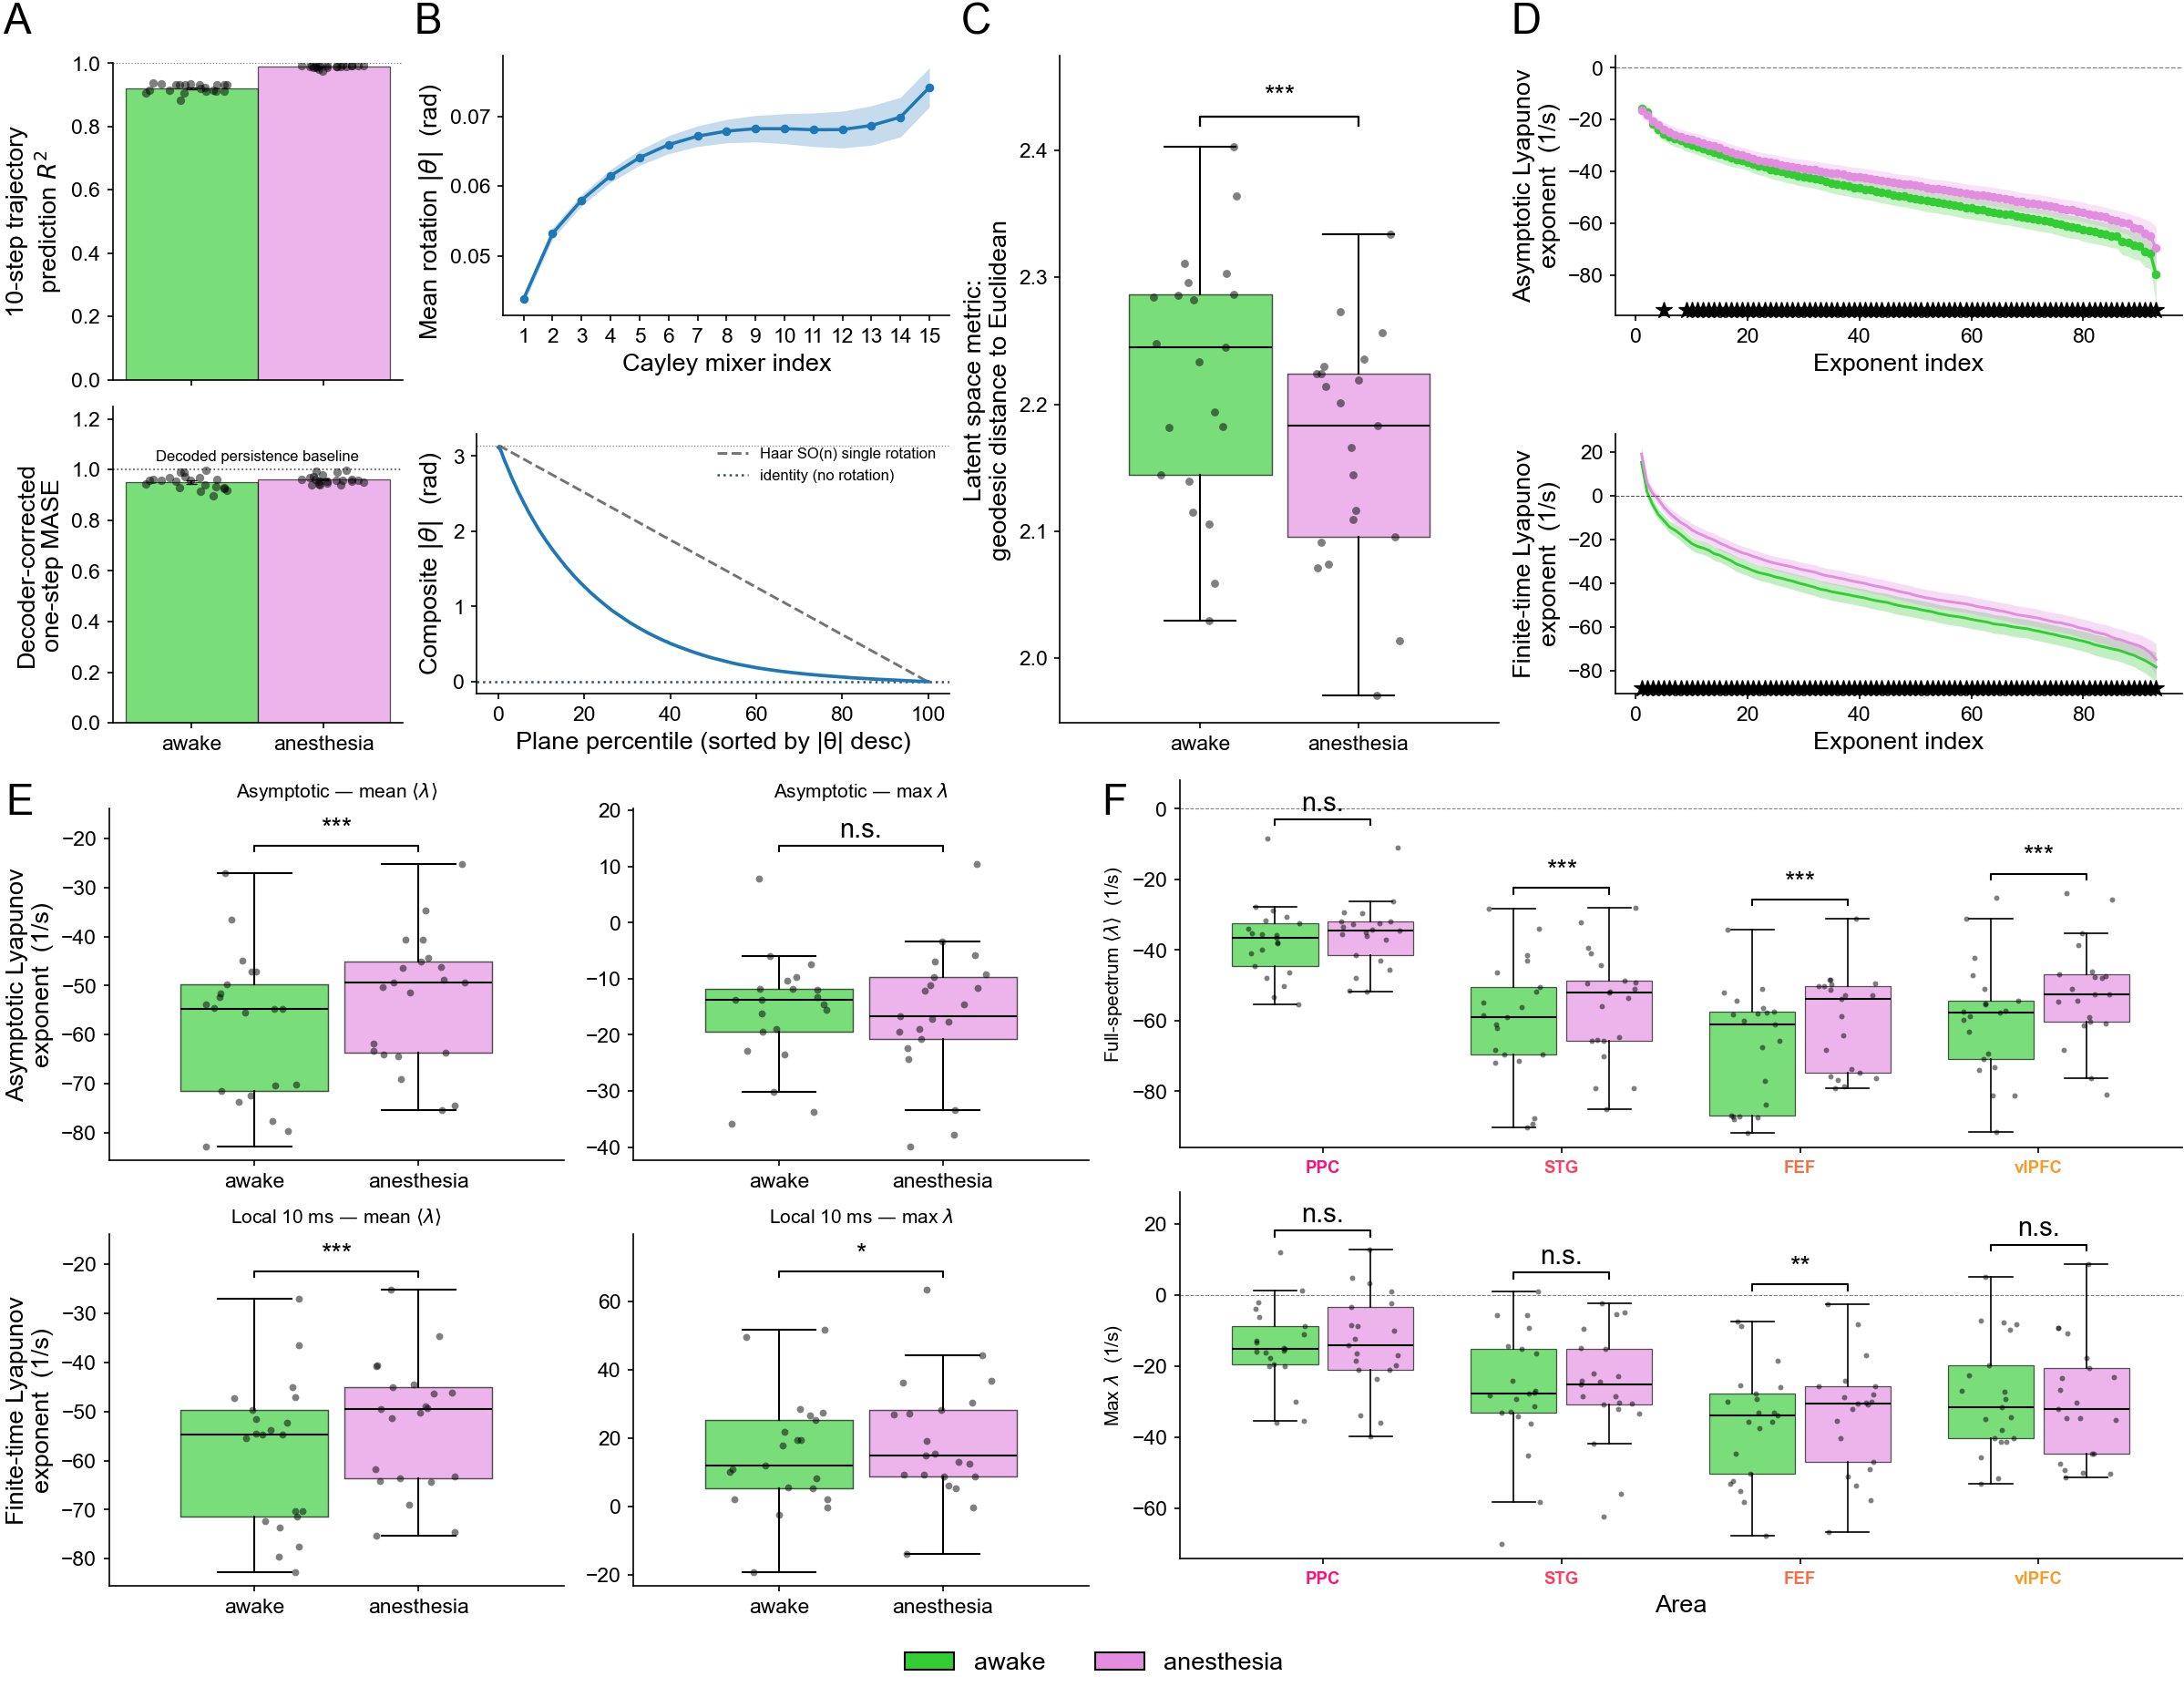
\includegraphics[width=\linewidth]{figures/interareal-control/fig_neural_lyap.png}
\caption[Trajectory prediction, encoder geometry, and Lyapunov spectra under propofol]{\textbf{Trajectory prediction, encoder geometry, and Lyapunov spectra under propofol} ($n=21$ sessions). (A)~Per-session 10-step $R^{2}$ and decoder-corrected one-step MASE, awake vs.\ anesthesia. (B)~Mean per-Cayley-layer rotation angle through encoder depth, between identity ($\theta=0$) and the Haar SO($n$) reference. (C) Geodesic distance from identity of the composite encoder Jacobian per session, awake (larger; more warped metric) vs.\ anesthesia ($p<0.001$). (D)~Full asymptotic (top) and 10-ms FTLE (bottom) Lyapunov spectra per session, sorted descending. (E)~Boxplots of asymptotic mean and max exponents and of 10-ms FTLE mean and max exponents. (F)~Per-area within-area asymptotic mean (top) and max (bottom) exponents per session for PPC, STG, FEF, vlPFC; sign-agree-gated significance annotated.}
\label{fig:interareal-control-neural-lyap}
\end{figure}

Per-area asymptotic Lyapunov exponents qualitatively reproduce the shift found at the full system level (Figure~\ref{fig:interareal-control-neural-lyap}F). Notably, PPC had the most unstable dynamics both in the awake and anesthetic states (paired two-sided Wilcoxon signed-rank with HL median paired difference, PPC $-$ other area, $n=21$ sessions; HL $\Delta$ ranging from $+16.2$ to $+28.6$~(1/s) across all six comparisons and all $p\leq 3\!\times\!10^{-6}$).

\subsection{Propofol anesthesia reduces directional reachability and controllability}
\label{sec:interareal-control-control}

We next sought to characterize how propofol anesthesia changes interareal reachability and controllability. We computed the directional reachability and controllability Gramians for each condition using the learned Jacobians. We report both the reachability and controllability Gramians computed over 10 millisecond horizons. Each gramian measures the influence of area $\beta$ on area $\alpha$ through the time-dependent coupling, defined by $\mathbf{J}^{\beta\to\alpha}$. For $\beta=\alpha$, $\mathrm{tr}(\mathbf{W}^{\alpha\alpha}_r) = \int_{t_0}^{t_1} \|\partial_\tau \boldsymbol{\Phi}_\alpha(t_1, \tau)\|_F^2\, d\tau$ and $\mathrm{tr}(\mathbf{W}^{\alpha\alpha}_c) = \int_{t_0}^{t_1} \|\partial_\tau \boldsymbol{\Phi}_\alpha(t_0, \tau)\|_F^2\, d\tau$: the integrated squared Frobenius norms of how the within-area state-transition matrices evolve with the integration time. This can be interpreted as the persistence of area $\alpha$'s own state through its within-area dynamics, either forward (for the reachability gramian) or backward (for the controllability gramian), and provides a natural baseline for comparing the trace magnitudes.

\begin{figure}[ht!]
\centering
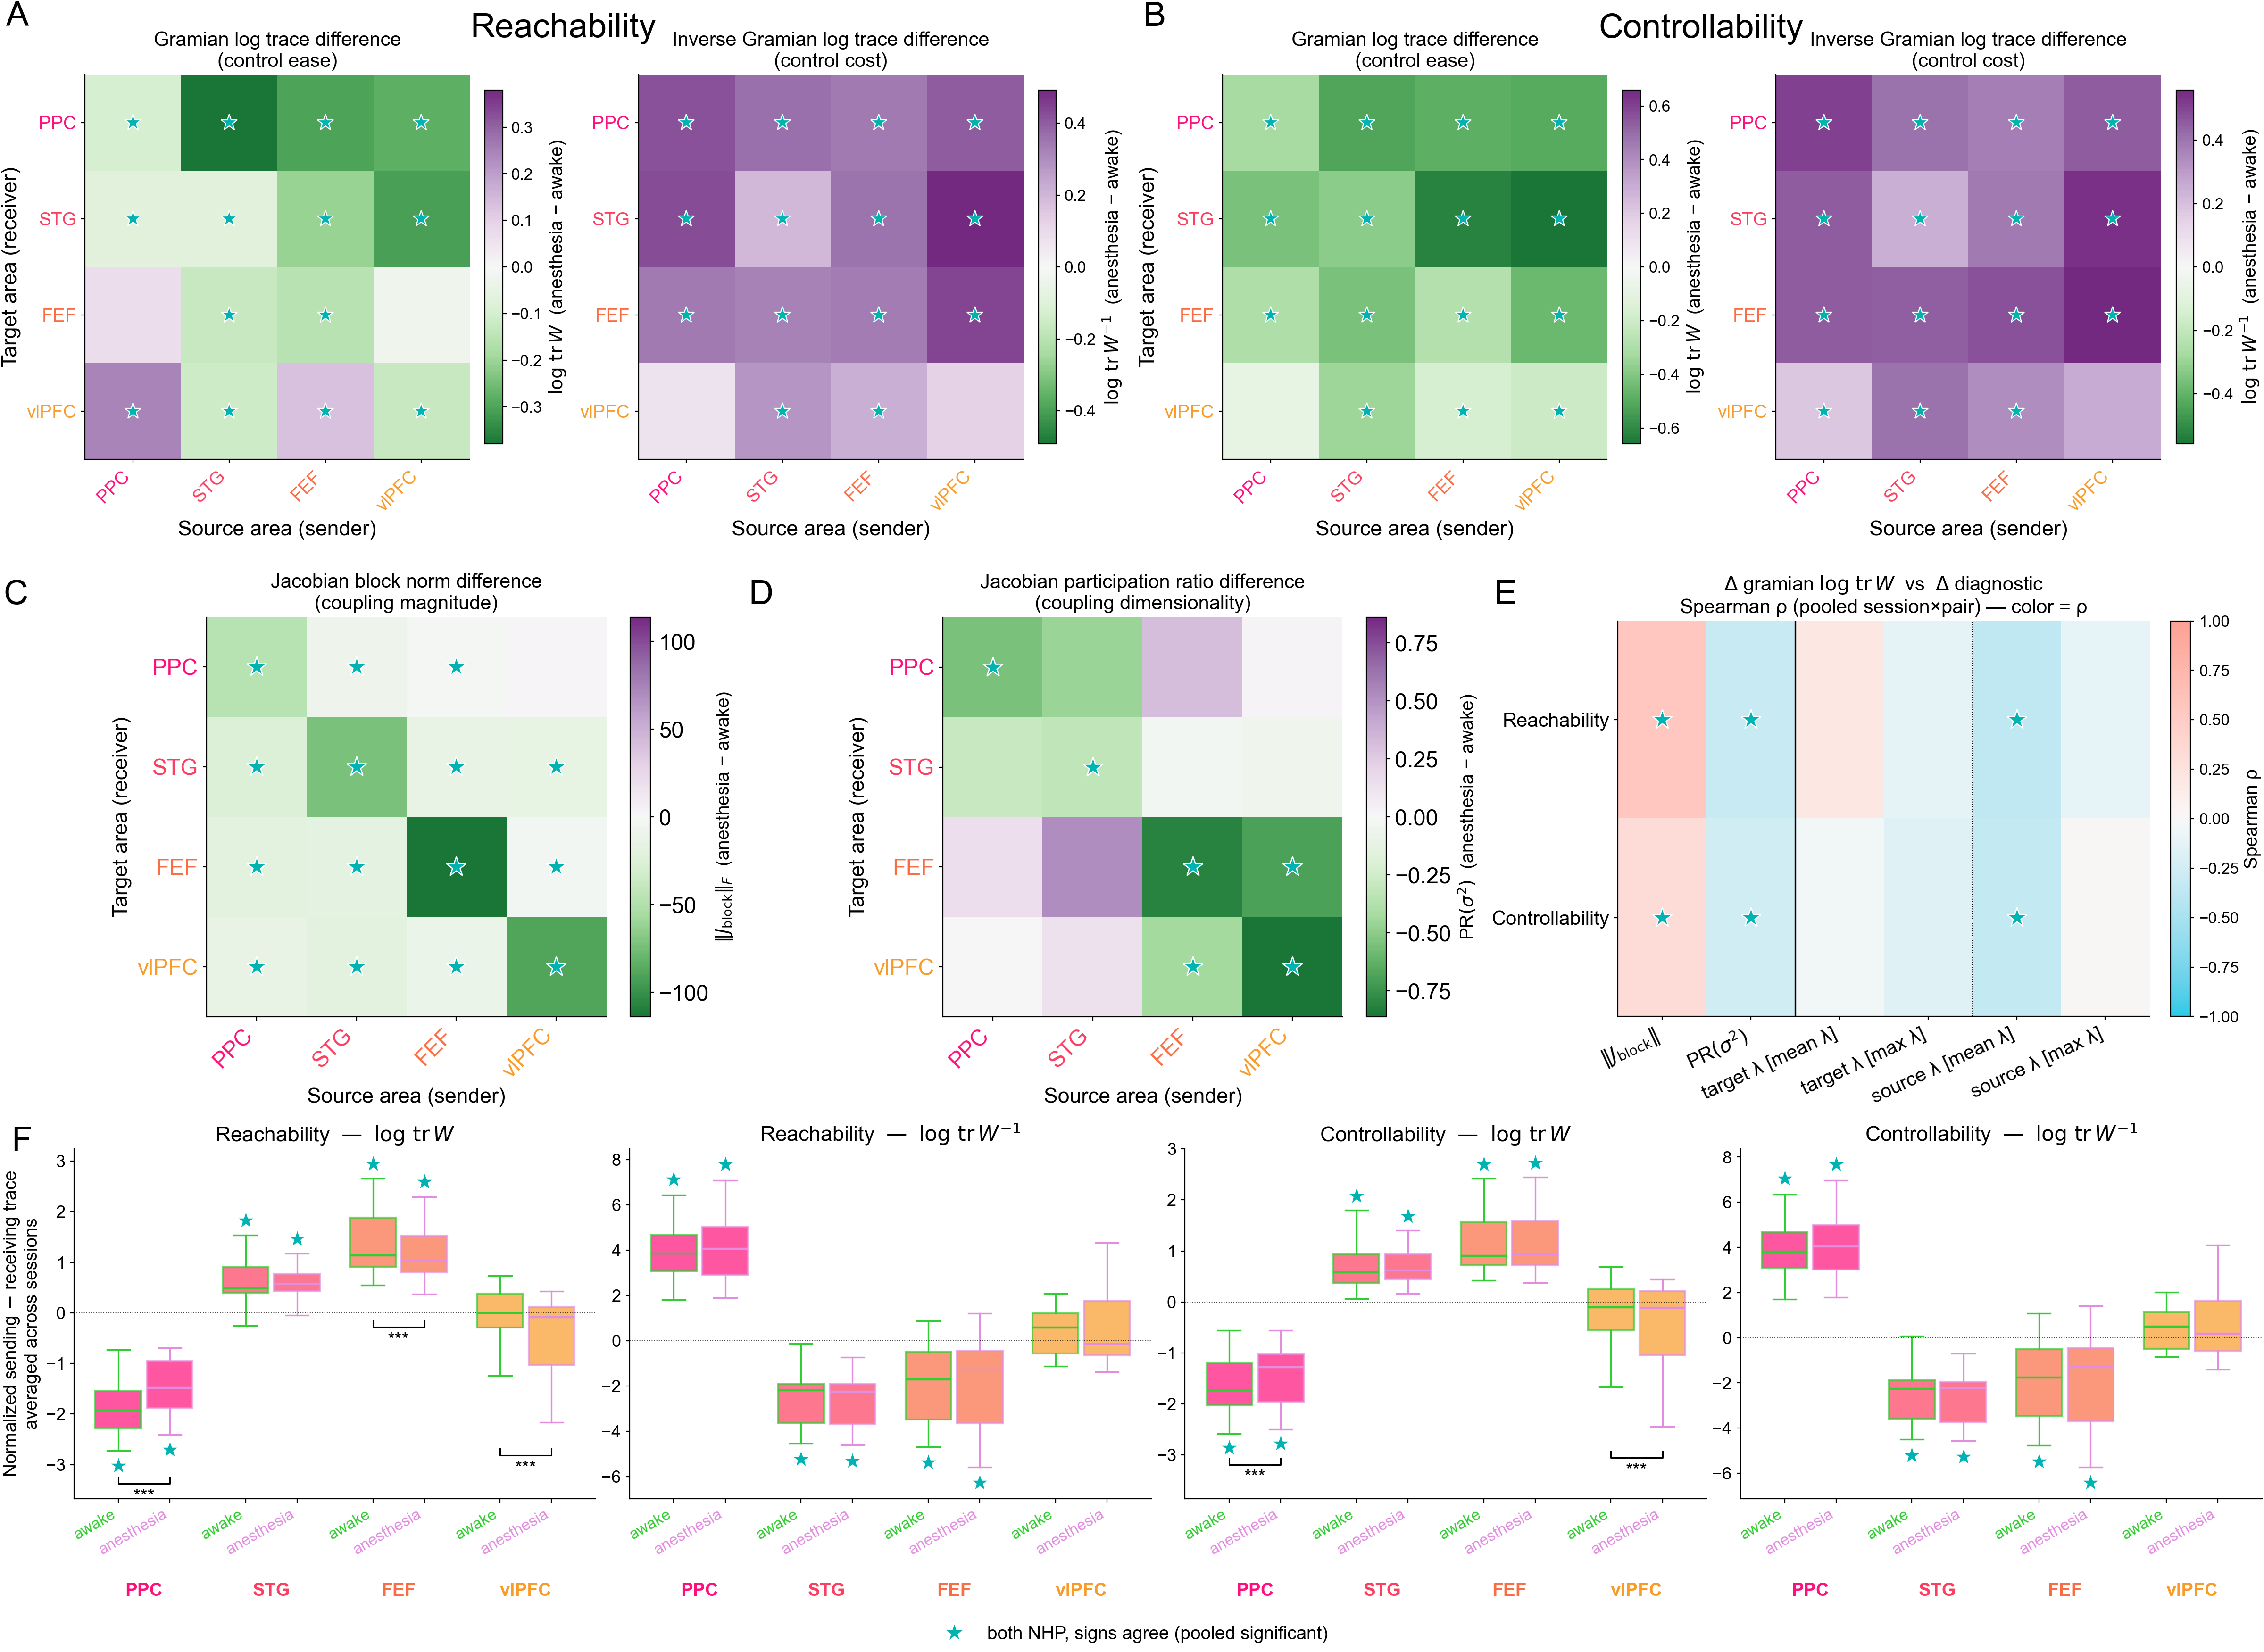
\includegraphics[width=\linewidth]{figures/interareal-control/fig_neural_control.png}
\caption[Directional reorganization of interareal control under propofol]{\textbf{Directional reorganization of interareal control under propofol} ($n=21$ sessions). (A)~$4\!\times\!4$ source--target heatmaps of pooled anesthesia$-$awake differences in reachability $\log\mathrm{tr}\,\mathbf{W}$ (left) and $\log\mathrm{tr}\,\mathbf{W}^{-1}$ (right); stars mark cells passing the sign-agree $+$ BH-FDR gate at $q<0.05$. (B)~Same for controllability. (C)~Jacobian block Frobenius-norm differences. (D)~Block participation-ratio differences. (E)~Spearman correlation between Gramian-change cells and block-norm/PR-change cells. (F)~Per-area net send$-$receive axis normalized by diagonal within-area measure across all four metrics, placing PPC at the receiver end, FEF/STG at the sender end, vlPFC balanced. }
\label{fig:interareal-control-neural-control}
\end{figure}

Reachability was broadly decreased under anesthesia, both when considering the easiest directions of control (Figure~\ref{fig:interareal-control-neural-control}A, left, trace; paired two-sided Wilcoxon signed-rank with HL median paired difference, anesthesia $-$ awake, $n=21$ sessions, per-pair Benjamini--Hochberg FDR across the 16 directed pairs with a per-NHP sign-agreement gate at $q<0.05$: log-trace decreased in 12/16 pairs with HL $\Delta$ ranging from $-0.40$ to $-0.07$ log-units) and the most difficult directions of control (Figure~\ref{fig:interareal-control-neural-control}A, right, inverse trace; same protocol: inverse log-trace increased in 14/16 pairs with HL $\Delta$ ranging from $+0.15$ to $+0.50$ log-units, all $q\leq 3.4\!\times\!10^{-4}$). Notably, the reachability along the most manipulable directions became \textit{easier} under anesthesia for the interactions involving both PPC and FEF driving vlPFC (PPC$\to$vlPFC: HL $\Delta=+0.24$ [95\% CI $+0.08$, $+0.41$], $p=0.013$, $q=0.017$; FEF$\to$vlPFC: HL $\Delta=+0.13$ [95\% CI $+0.02$, $+0.23$], $p=0.019$, $q=0.024$).

Controllability was also broadly decreased under anesthesia, both when considering the easiest directions of control (Figure~\ref{fig:interareal-control-neural-control}B, left, trace; paired two-sided Wilcoxon signed-rank with HL median paired difference, anesthesia $-$ awake, $n=21$ sessions, per-pair Benjamini--Hochberg FDR across the 16 directed pairs with a per-NHP sign-agreement gate at $q<0.05$: ctrl log-trace decreased in 15/16 pairs with HL $\Delta$ ranging from $-0.67$ to $-0.18$ log-units, all $q\leq 1.1\!\times\!10^{-2}$) and the most difficult directions of control (Figure~\ref{fig:interareal-control-neural-control}B, right, inverse trace; same protocol: ctrl inverse log-trace increased in 15/16 pairs with HL $\Delta$ ranging from $+0.21$ to $+0.54$ log-units, all $q\leq 4.0\!\times\!10^{-3}$).

These disruptions in reachability and controllability are most evident at the short time horizon (10 milliseconds) presented here. At longer horizons, the intrinsic dynamics (more destabilized under anesthesia) increasingly dominate the Gramians over the interareal coupling. When the target system is less stable, reachability becomes easier and controllability becomes harder. Thus, over longer horizons, reachability becomes easier under anesthesia (particularly for projections to PPC and STG), while the controllability reduction instead deepens (Appendix~\ref{supp:interareal-control-horizons}). This illustrates that a reduction in the ability to drive posterior areas manifests on shorter horizons (10, 20, and 100 milliseconds), while on longer timescales (1 second) the intrinsic instability of the target area dynamics leads to greater reachability.

\subsection{Anesthesia reduces coupling strength and local coupling dimensionality}
\label{sec:interareal-control-block-norm}

To probe the influence of anesthesia on coupling strength, we analyzed how anesthesia changes both the Frobenius norm of the cross-area and within-area Jacobian blocks ($\Delta\log\mathrm{tr}\,\mathbf{W}$ and $\Delta\|\mathbf{J}_{\mathrm{block}}\|$, the difference in Frobenius norm of the coupling blocks between states), and the participation ratios of these blocks ($\Delta\mathrm{PR}(\sigma^2)$, i.e. change in the participation ratio of the singular values of $\mathbf{J}_{\mathrm{block}}\mathbf{J}_{\mathrm{block}}^T$). We found that the Frobenius norm of the Jacobian blocks broadly decreased during anesthesia, indicative of reduced coupling strength between areas (Figure~\ref{fig:interareal-control-neural-control}D; paired two-sided Wilcoxon signed-rank with HL median paired difference, anesthesia $-$ awake, per-pair Benjamini--Hochberg FDR across the 16 directed pairs with a per-NHP sign-agreement gate at $q<0.05$, $n=21$ sessions: 13/16 pairs decreased with HL $\Delta$ ranging from $-119$ to $-8$, all $q\leq 1.3\!\times\!10^{-4}$). The participation ratios (dimensionality) of the Jacobian blocks showed more mixed results. Within frontal (FEF, vlPFC) and within posterior (PPC, STG) cortices anesthesia decreased coupling dimensionality (Figure~\ref{fig:interareal-control-neural-control}E). All four within-frontal pairs decreased significantly (same protocol applied to PR$(\sigma^2)$; HL $\Delta$ ranging from $-0.85$ to $-0.37$, all $q\leq 4.3\!\times\!10^{-3}$) and within posterior, both diagonal pairs PPC$\to$PPC and STG$\to$STG decreased ($\Delta=-0.52$, $q=7.1\!\times\!10^{-5}$ and $\Delta=-0.22$, $q=7.7\!\times\!10^{-4}$). For the frontal-to-posterior and posterior-to-frontal couplings, the results were not significant but tended to be higher during anesthesia. This suggests that anesthesia decouples more closely related areas but potentially creates more diffuse, albeit weakened, couplings across more distant areas. To formalize this within-versus-between contrast, we computed for each session the mean $\Delta\mathrm{PR}(\sigma^2)$ across within-cluster pairs minus the mean across between-cluster pairs and tested whether this contrast differed from zero across the cohort: 20/21 sessions had a more-negative within-cluster mean than between-cluster mean (sign-agree across NHPs, with pooled HL contrast $\Delta=-0.69$ [95\% CI $-0.94$, $-0.43$], paired two-sided Wilcoxon signed-rank $p=9.5\!\times\!10^{-6}$).

\subsection{Changes in reachability and controllability are driven by multi-factorial anesthesia-induced effects}
\label{sec:interareal-control-multifactor}

Finally, we assessed how various factors explain changes in reachability and controllability. We correlated the changes in Gramian traces with changes in block-norm and participation-ratio, as well as with changes in target and source-area Lyapunov exponents across conditions (Figure~\ref{fig:interareal-control-neural-control}F). We found that the correlation was weak and inconsistent, indicating that directional control reorganization is driven by input-direction alignment beyond cross-coupling scale alone. The traces are positively correlated with block-norm changes, indicating that coupling magnitude is a significant contributor to control ease (Spearman $\rho$ between $\Delta\log\mathrm{tr}\,\mathbf{W}$ and $\Delta\|\mathbf{J}_{\mathrm{block}}\|$ pooled across session $\times$ pair, with per-NHP sign-agreement gate and session-clustered permutation testing: reach $\rho=+0.56$, $p=1.0\!\times\!10^{-4}$; ctrl $\rho=+0.32$, $p=1.0\!\times\!10^{-4}$; both sign-agree). Interestingly, they are negatively correlated with the participation ratio changes, indicating that more diffuse coupling might actually impede control along the most essential directions (Spearman $\rho$ between $\Delta\log\mathrm{tr}\,\mathbf{W}$ and $\Delta\mathrm{PR}(\sigma^2)$, same protocol: reach $\rho=-0.31$, $p=1.0\!\times\!10^{-4}$; ctrl $\rho=-0.25$, $p=0.044$; both sign-agree). Overall, the correlations were relatively weak, reflecting that directional control depends on a multitude of factors that include the coupling strength and dimensionality, as well as the dynamic stability of the source and target areas, and the alignment of the source projection with the directions of flow in the target area.

\subsection{Anesthesia disrupts the hierarchy of cortical organization into senders and receivers}
\label{sec:interareal-control-area-roles}

To evaluate area-wise patterns, we first normalized each off-diagonal cross-area gramian measure by the within-area measure of the target area. We then computed the column-wise mean (corresponding to average sending capability) and row-wise mean (corresponding to average receiving capability). This gives us a per-area measure of the average sending capability relative to receiving capability within each condition (Figure~\ref{fig:interareal-control-neural-control}C). We found that across both awake and anesthesia PPC was consistently more of a receiving area, while STG and FEF were consistently more sending areas. vlPFC was balanced, indicative of its role as a hub (one-sample two-sided Wilcoxon signed-rank vs $0$ with per-NHP sign-agreement gate, $n=21$ sessions: PPC's net was significantly receiver-side in all four metrics in both conditions with all $p\leq 9.5\!\times\!10^{-7}$; STG and FEF were significantly sender-side in all four metrics in both conditions with STG all $p\leq 1.9\!\times\!10^{-6}$, FEF all $p\leq 4.3\!\times\!10^{-4}$, both sign-agree; and vlPFC failed the per-NHP sign-agreement gate in all cells). While the roles were preserved across conditions, anesthesia tended to push areas more toward a balanced regime (sending capability equivalent to receiving capability), thus disrupting cortical organization. PPC and FEF, the two areas with the most extreme awake-state roles, both shifted toward balance under anesthesia (paired two-sided Wilcoxon signed-rank with HL median paired difference, anesthesia $-$ awake, per-NHP sign-agreement gate, $n=21$ sessions; reach log-trace panel: PPC $\Delta=+0.41$ [95\% CI $+0.26$, $+0.56$], $p=9.5\!\times\!10^{-7}$; FEF $\Delta=-0.13$ [$-0.21$, $-0.07$], $p=6.7\!\times\!10^{-6}$). vlPFC, near-balanced when awake, drifted further into a receiver-like configuration ($\Delta=-0.29$ [$-0.41$, $-0.20$], $p=9.5\!\times\!10^{-7}$). The same qualitative pattern held for the controllability log-trace panel for PPC ($\Delta=+0.17$, $p=1.3\!\times\!10^{-4}$) and vlPFC ($\Delta=-0.14$, $p=1.8\!\times\!10^{-5}$).

\section{Discussion}
\label{sec:interareal-control-discussion}

Our results show that anesthesia decreases the ability of areas to control each other, both in terms of driving towards novel states and stabilizing along existing trajectories. We reproduced earlier results, showing that propofol anesthesia induces broad spectrum destabilization of neural dynamics. While the destabilization was most pronounced in PPC, it was pervasive across all areas. Interestingly, despite decreased stability relating to increased reachability ease in the absence of other changes, we found that reachability broadly decreased in anesthesia. This suggests that at the time horizon of 10 milliseconds considered in the main text, the decreased stability in target areas could not compensate for the reduction in coupling strength also observed. This again highlights that changes in reachability and controllability were driven by multi-factorial anesthesia-induced effects, including changes in coupling strength and dimensionality, as well as the dynamic stability of the source and target areas.

\insettitle{Paradoxical excitation.} Notably, the directional interactions from PPC to vlPFC and from FEF to vlPFC showed surprising increases in reachability under anesthesia. These pathways could potentially be interpreted as a mechanism of the paradoxical excitation observed during propofol anesthesia. Paradoxical excitation is characterized by an increase in abnormal movements as well as sensory hallucinations.\cite{Jeong2011-mr, McCarthy2008-pe, Sneyd1992-ku} Thus, it may be that the increased ease with which PPC and FEF can drive vlPFC under anesthesia may lead to the observed spurious movements and sensory hallucinations prior to the onset of loss of consciousness.

\insettitle{Reduced coupling magnitude during anesthesia.} Our finding of reduced coupling magnitude during anesthesia aligns with previous findings of reduced synchrony and network integration during propofol infusion.\cite{Lewis2012-bs, Bardon2025-zi, Li2026-nh, Huang2024-px, Liang2025-li, Wilsenach2025-zy, Castro2024-dr, Luppi2025-oa, Luppi2024-yl, Alkire2008-zy, Boveroux2010-pn, Demertzi2019-gz, Song2015-lm, Lee2018-su, Malekmohammadi2018-oa, Ensel2024-cg, Tauber2023-sp, Franks2008-ej} Furthermore, the finding that coupling dimensionality decreases locally (within frontal and posterior areas) but decreases more globally (across frontal and posterior areas) aligns with recent findings of reduced synchrony within hemisphere but increased synchrony across hemispheres.\cite{Bardon2025-zi}

\insettitle{Neuropsychiatric conditions.} We also note that the latent JacobianODE pipeline leveraged in this work was agnostic to both the recording modality and the nature of the data (anesthetic infusion) and could be applied in a wide range of settings. Neuropsychiatric conditions, in particular, present a compelling setting in which to explore the application of nonlinear interareal control analyses. Neural control has been shown to be relevant in schizophrenia,\cite{Li2023-zg, Mahadevan2023-bw,Zoller2021-ib} and epilepsy,\cite{He2022-fp}, and a lack of goal-directed control has been identified across multiple psychiatric conditions.\cite{Gillan2016-fm} Additionally, dysregulation of the cortico-basal ganglia-thalamocortical loop has been associated with a wide range of neuropsychiatric conditions that includes addiction, attention-deficit/hyperactivity disorder, Parkinson’s, and many others.\cite{Redish2004-jw, Frank2007-dx, Maia2011-ca} Notably, these conditions all involve a lack of control in some form, suggesting this might be a compelling setting in which to look for control theoretic biomarkers and treatment predictors.

\insettitle{Interventional control.} Prior work has shown that JacobianODE models can be used to directly control synthetic neural models to produce desired behaviors.\cite{Eisen2025-wt} This raises the possibility of using the latent JacobianODE pipeline for interventional control in both basic science and clinical settings, such as transcranial magnetic stimulation (TMS) and deep brain stimulation (DBS).\cite{Siddiqi2020-en, Siddiqi2024-su, Krauss2021-iv,Tiruvadi2022-bj,Alagapan2023-yd} Given an appropriate mapping from stimulus to brain activity, the control inputs could actually be computed in stimulus space, obviating the need for technologically complex manipulation.\cite{Bashivan2019-yv}

\subsection{Future directions}

We validated that the latent JacobianODE method is capable of capturing relative changes in reachability and controllability from partial observation in the task-trained RNN. However, it should be determined whether the model is capable of recapitulating these relative changes when there are more than two subsystems present.

A challenge of the latent Jacobian estimation pipeline is the need to pick the intrinsic dimensionality of the latent dynamics $d_{\text{dyn}}$. In the present work, we err on the side of caution and pick a dimensionality sufficient to explain 99\% of the variance in principal component space in the data. However a nonlinear method of intrinsic dimensionality estimation that yields tighter bounds to the true intrinsic dimensionality of the system would both save compute (as higher dimensions require larger models) and likely yield improved Jacobian estimation. An outstanding possibility not explored in this work is to use the learned geometry of the encoder (c.f., the induced Riemannian metric on the latent space) to infer the true number of directions that are relevant for the latent manifold.

Furthermore, the models fit to neural data surpassed the decoder-corrected persistence baseline, but did not adequately reproduce the asymptotic dynamics of the system. To do so, a compelling alternative is to leverage the nonautonomous extension of the JacobianODE framework suggested in the initial presentation of the method.\cite{Eisen2025-wt} Incorporating this change would vastly increase the expressivity of the model and potentially lead to more effective models of neural dynamics.

While we focus here on control, we note that a wide range of tools have been developed and harnessed to study interareal interactions in neural data.\cite{Kass2023-dt, Semedo2020-qz} They include methods based on reduced rank regression,\cite{Semedo2019-ml, MacDowell2023-da} recurrent neural network models of neural dynamics,\cite{Perich2021-sq, Perich2020-ii, Andalman2019-ks, Pinto2019-ak, Kleinman2021-dz} Gaussian-process factor analysis,\cite{Gokcen2022-gu} canonical correlation analysis,\cite{Ebrahimi2022-ed, Rodu2018-bb} convergent cross mapping,\cite{Ye2015-ma, Sugihara2012-be} switching dynamical systems,\cite{Karniol-Tambour2023-ti, Glaser2020-kz} granger causality,\cite{Bressler2011-dp, Seth2015-be} and point process models.\cite{Chen2022-pm} A complete analysis should consider how these existing metrics vary with propofol anesthesia to provide a more comprehensive picture of changes in interareal interactions during anesthetic-induced unconsciousness.